% Dealerless Orca Ring-LPN proposal, v2.17 (2026-08-17): current internal/advisor checkpoint
% Version 2.17 (2026-08-17): controlled CNN2/CNN3 matrix, hardened transport, and complete current evidence integration
%   1) problem overview  2) motivation (dealerless + GPU)
%   3) proposed design   4) experiment setup
% All "Figure 2" references to BCG+20 renamed to "BCG+20 generator";
% this document now contains its own figures.
% Numbers: measured values are regenerated from the current artifact CSVs;
% the distributed-keygen cost table is derived per DPF tree, including three
% scalar OLEs per tree and the bootstrap condition 3 c^2 t^2 < n.
\documentclass[11pt]{article}

\usepackage[margin=1in]{geometry}
\usepackage{amsmath,amssymb,amsthm}
\usepackage{booktabs}
\usepackage{array}
\usepackage{xcolor}
\usepackage{tikz}
\usetikzlibrary{positioning,arrows.meta,calc}
\usepackage{hyperref}

\hypersetup{
  colorlinks=true,
  linkcolor=blue!60!black,
  citecolor=blue!60!black,
  urlcolor=blue!60!black
}

\emergencystretch=1.5em % long unbreakable \texttt identifiers; avoid overfull lines

\newcommand{\Z}{\mathbb{Z}}
\newcommand{\Ring}{\mathcal{R}}
\newcommand{\ServerZero}{\mathsf{P}_0}
\newcommand{\ServerOne}{\mathsf{P}_1}
\newcommand{\bw}{\mathsf{bw}}
\newcommand{\modtwo}{\Z_{2^{\bw}}}
\newcommand{\Q}{Q}   % composite CRT modulus Q = p_0 p_1 (renamed from M to avoid clashing with the layer dimension M)
\newcommand{\dpfd}{d_{\mathrm{DPF}}} % DPF tree depth; distinct from CRT limbs L and conversion bit length \ell

\title{Dealerless GPU Preprocessing for Orca Linear Layers\\
\large Internal/Advisor Technical Checkpoint}
\author{Alp Caglar}
\date{August 17, 2026}

\begin{document}
\maketitle

\begin{center}
\fbox{\begin{minipage}{0.92\linewidth}\small
\textbf{Circulation boundary.} Internal/advisor checkpoint only; not a
submission candidate. Final authorship, contributor credit, permission to
reuse any private-project overlap, and disclosure language require an explicit
professor/owner ruling before external circulation.
\end{minipage}}
\end{center}

\begin{abstract}
We implement a two-process GPU preprocessing path that replaces Orca's trusted
dealer for forward linear layers at unpinned Ring-LPN feasibility parameters.
Party-local sparse noise feeds distributed DPF generation, Ring-LPN OLE,
noncircular Ring-OLE-output bootstrap, exact $\Z_Q\!\to\!\Z_{2^\bw}$
conversion, stock-format key serialization, and unchanged Orca FC/Conv2D
consumers. The default SCI/IKNP focused suite and a separate opt-in EMP-Silent
rerun each pass the same five q64/q128 cases and sixteen rejection controls;
the latter is independently unreviewed correctness/accounting evidence only.
The controlled source-manifest matrix covers both CNN2 FC layers and the CNN3
FC scale point. Every layer passes one warmup plus ten measured trials. On a
quiescent RTX 5000 Ada selected per sample for both the protocol critical path
and subsequent stock dealer, median setup-included preprocessing/stock-dealer
ratios are $879.30\times$ for CNN2's two FC layers in aggregate and
$60.32\times$ for CNN3 FC5. These same-host feasibility results are
a controlled negative comparison, not a speedup or security claim.
A source-native terminal FC/Conv2D application also passes nonzero input-share
and public-bias checks; the extracted stock helpers pass signed/wrapping clear
oracles. Arbitrary multi-layer mask-state chaining remains open.

A source-bound known-zero control separately composes all 21 fresh linear
records through the exact 62-item ResNet18 stream. Its trusted test-only
adapter reads both parties' mask states, supplies both truncation
successor-mask shares and remask/terminal material, and generates the nonlinear
keys. This proves graph/state compatibility only---not dealerless nonlinear
preprocessing, private/trained inference, or full-model performance. Mutual
HMAC-SHA256 authenticates endpoint roles and invocation context before local
preflight, but later protocol bytes have no per-message integrity. The
exercised source tuple $(n,c,t)=(8192,2,8)$ and full-graph execution override
$(262144,2,8)$ are correctness points, not concrete-security pins. Authenticated
distinct-host execution, a compatible dealerless baseline, qualified
independent review, clean-clone evidence, and final release identities remain
open. Accordingly, this document is an internal technical checkpoint, not a
publication-ready security or systems result.
\end{abstract}

\paragraph{Artifact and claim discipline.}
Historical numerical claims use the retained manifests/CSVs named in
\S\ref{sec:baseline}; the September review experiment is separately identified
in \S\ref{sec:worker-review}. Historical source, binary, schema, and evidence digests are checked by
the release gate. q64/q128 denote one/two approximately 62-bit CRT limbs, not
security levels. ``Authenticated'' for the current same-host measurements means
only the preflight endpoint/context handshake; the conditional theorem still
assumes authenticated channels.

\section{Executive status: what is implemented, what is not}

\paragraph{Thesis.}
This work has two deliberately separate results:
\emph{(i)} an executable forward-linear preprocessing pipeline without a
trusted dealer in the stated random-oracle model, validated by unchanged Orca
consumers; and \emph{(ii)} a known-zero full-graph compatibility control whose
nonlinear/truncation state is explicitly trusted. The system result is the
composition, GPU/system design, fail-closed state machinery, and evidence
boundary; Ring-LPN, DPF, OT/OLE, conversion, Beaver multiplication, and Orca
remain prior components. No concrete Ring-LPN parameter or compatible
dealerless-PCG performance comparison is established.

\section{Problem overview: Orca's preprocessing and its trusted dealer}
\label{sec:problem}

\subsection{Background: Orca in one page}
\label{sec:orca}

Orca~\cite{jawalkar2024orca} is a two-party secure computation (2PC) system
for neural-network training and inference, engineered around GPUs. Two servers
$\ServerZero$ and $\ServerOne$ hold additive secret shares of all inputs,
weights, and activations; neither learns anything beyond its own shares.
Like most practical 2PC systems, Orca splits work into an input-independent
\emph{preprocessing} (offline) phase that generates correlated randomness, and
a fast \emph{online} phase that consumes it:

\begin{itemize}
\item \textbf{Linear layers} (convolutions, fully-connected/FC layers) consume
  \emph{Beaver-triple--style matrix keys}: for a layer multiplying an
  $M{\times}K$ matrix by a $K{\times}N$ matrix, the parties need shares of
  random masks $A, B$ and of the product terms that make the masked
  multiplication identity work. Online, each party opens masked operands and
  runs the local computation implemented by \texttt{gpuMatmulBeaver}.
\item \textbf{Nonlinear layers} (ReLU, truncation) consume function secret
  sharing (FSS) keys --- distributed comparison functions (DCFs) --- with a
  different structure.
\end{itemize}

In stock Orca \emph{both} kinds of keys are produced by a \textbf{trusted
dealer}: a third machine that samples every mask, computes every correlated
value, and ships each party its key files (Figure~\ref{fig:dealer}).

\begin{figure}[t]
\centering
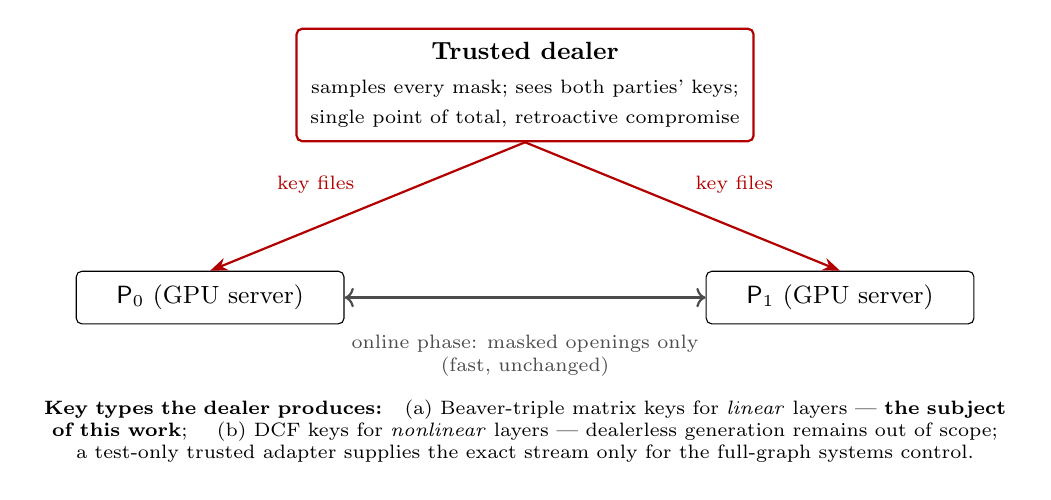
\begin{tikzpicture}[
  box/.style={draw, rounded corners=2pt, align=center, font=\small, inner sep=5pt},
  arr/.style={-{Stealth[length=2.2mm]}, thick},
  lbl/.style={font=\scriptsize, align=center}
]
\node[box, draw=red!70!black, thick, minimum width=52mm]
  (dealer) at (0,0) {\textbf{Trusted dealer}\\[1pt]
  \scriptsize samples every mask; sees both parties' keys;\\
  \scriptsize single point of total, retroactive compromise};
\node[box, minimum width=34mm] (p0) at (-40mm,-27mm) {$\ServerZero$ (GPU server)};
\node[box, minimum width=34mm] (p1) at (40mm,-27mm) {$\ServerOne$ (GPU server)};
\draw[arr, red!70!black] (dealer.south) -- (p0.north)
  node[lbl, midway, above left=0.5mm] {key files};
\draw[arr, red!70!black] (dealer.south) -- (p1.north)
  node[lbl, midway, above right=0.5mm] {key files};
\draw[arr, <->, black!70] (p0.east) -- (p1.west)
  node[lbl, midway, below=3.5mm] {online phase: masked openings only\\ (fast, unchanged)};
\node[lbl, text width=124mm] at (0,-44mm) {
  \textbf{Key types the dealer produces:}\quad
  (a) Beaver-triple matrix keys for \emph{linear} layers --- \textbf{the
  subject of this work}; \quad (b) DCF keys for \emph{nonlinear} layers ---
  dealerless generation remains out of scope; a test-only trusted adapter
  supplies the exact stream only for the full-graph systems control.};
\end{tikzpicture}
\caption{Orca's preprocessing today. The dealer is trusted with every secret
of the offline phase. This proposal removes it for the linear-layer keys;
the online phase is never modified.}
\label{fig:dealer}
\end{figure}

\subsection{Current status of our pipeline}
\label{sec:status}

Over the preceding milestones this project built, and validated on GPUs, a
preprocessing pipeline that produces Orca's FC-layer keys from \emph{Ring-LPN
pseudorandom correlation generators} rather than from a dealer's coin flips.
The pipeline (Figure~\ref{fig:pipeline}; components defined in
\S\ref{sec:design}) already works end-to-end with \emph{real} correlation
generators --- not idealized stand-ins --- at both supported modulus widths,
and its output keys are validated by the strongest referee available: Orca's
\emph{unchanged} online code reconstructs the correct products
(\S\ref{sec:baseline} gives the measured evidence).

\subsection{Historical gaps and current boundary}
\label{sec:gaps}

The original one-process transcript had four dealer/security gaps. The live
forward artifact closes the first three at the executable level; the fourth
still blocks a deployable security claim. Dealerless nonlinear preprocessing
remains outside the theorem; a narrow trusted-adapter systems control now
executes the stock nonlinear consumers.

\begin{description}
\item[G1 --- Centralized SPFSS setup: closed in the live path.] Each process
  samples only its own sparse noise, participates in distributed GPU-AES DPF
  key generation, and expands only its own Ring-LPN share. The older
  one-process transcript retains \texttt{build\_spfss\_keys()} solely as a
  diagnostic/validation artifact; none of its timings are presented as live
  protocol measurements.
\item[G2 --- Exact share conversion: closed.]
  Batched edaBits, daBits, and Boolean triples from the selected OT backend
  implement exact $\Z_Q\to\Z_{2^\bw}$ conversion. The canonical and classifier
  suites use SCI/IKNP. A current separate EMP-Silent rerun passes the same five
  focused cases and sixteen controls with exact directional inventory
  exhaustion, but remains opt-in and independently unreviewed. The wrap bit is
  never opened; the simulator in \S\ref{sec:design-convert} proves privacy at
  the correlation boundary. The measured local runner first performs mutual
  HMAC-SHA256 endpoint/context establishment; later loopback bytes have no
  application-layer per-message integrity.
\item[G3 --- Randomness/RO separation: closed.]
  Private roots, masks, and noise come from each process's OpenSSL private
  DRBG. For every Ring-OLE correlation, $a_0=1$ is the unsent public identity
  polynomial. Each party exchanges four uniform 64-bit seed-share words; their
  XOR is one jointly sampled 256-bit public seed. The full 256-bit correlation
  scope and all public Ring-OLE parameters domain-separate SHAKE256 rejection
  sampling of every $(c-1)n$-coefficient tail, giving independent exact-uniform
  ring elements in the explicit random-oracle model rather than an
  information-theoretic coin-toss claim.
\item[G4 --- Security parameters: open.] The deployed $(c,t)=(2,8)$ values are
  feasibility parameters. The exact splittable Ring-LPN distribution and the
  two-CRT-limb composition have no reviewed concrete classical/quantum
  advantage bound or accepted parameter pin.
\item[G5 --- Scope.] Stateful training and dealerless nonlinear DCF key
  generation are not implemented. The proved/exercised security scope remains
  forward FC. A separate source-bound known-zero systems control executes the
  complete stock ResNet18 graph with a trusted nonlinear key source;
  ``dealerless Orca'' without the forward-linear qualifier remains false.
\end{description}

\paragraph{Contributions.}
(1)~A live, trusted-dealer-free two-process forward-FC/Conv2D preprocessing
path in the stated random-oracle model, whose party-local outputs are consumed
by unchanged Orca code;
(2)~a source-specific exact algebraic coupling of distributed DPF correction
words to standard generation, complete role-specific batch simulators, and an
executable compatibility repair that bootstraps every post-base Phase-C product
from Ring-OLE output;
(3)~a tree-block GPU Phase-C implementation whose correctness and component
timings are retained without claiming an end-to-end speedup;
(4)~a hybrid-model privacy proof and live realization of exact
$\Z_Q\to\Z_{2^\bw}$ conversion;
(5)~a source-to-transcript map and conditional forward-FC theorem with explicit
leakage, assumptions, and nonclaims;
(6)~a source-manifest-derived CNN2/CNN3 forward-FC feasibility matrix with one
warmup and ten passing trials per layer and a same-physical-GPU,
quiescence-checked stock trusted-dealer comparator;
(7)~a fail-closed source-bound known-zero full-ResNet18 systems composition
using all 21 linear records and the exact 62-item stock stream; and
(8)~a manifest-bound clean-clone/container gate that rebuilds the paper and
canonical checks while rejecting source mutation and private-artifact
survivors. A final same-HEAD clean-clone execution remains a release gate.

The corrected three-product Phase C is a local compatibility bug fix, not an
independent novelty contribution. The canonical audit records chronology and
conceptual overlap with a private project's earlier correction of a leaky DPF
output layer; professor/contributor credit, permission, disclosure, and
private-project-overlap rulings remain explicitly open and must be settled
before external circulation. The point-DPF and Ring-LPN generator primitives
are prior work, not claimed as novel. This is feasibility evidence: the
controlled CNN2/CNN3 median setup-included preprocessing/dealer ratios are
$879.2970985824659\times$ and $60.3181599795375\times$, respectively.
Together with unprotected post-handshake local transport and unpinned Ring-LPN
parameters, these negative results are publication risks rather than
competitive-system evidence.
\section{Motivation: why dealerless, and why on GPUs}
\label{sec:motivation}

\subsection{Why remove the dealer}
\label{sec:motivation-dealer}

The dealer is the single point of \emph{total, retroactive} compromise: it
holds every mask of every computation, so one breach --- or one subpoena, or
one insider --- retroactively breaks the privacy of everything the two parties
ever computed. The trust assumption is also operationally awkward: in many
two-party deployments (two mutually distrusting companies; a hospital and an
ML provider) no mutually trusted third machine exists, and dealer key material
for training runs is measured in gigabytes that must be generated, stored, and
shipped securely. Removing the dealer replaces an institutional assumption
with a cryptographic one.

\subsection{Why pseudorandom correlation generators, and which one}
\label{sec:motivation-pcg}

A training run consumes correlated randomness for billions of secure
multiplications; any protocol paying per-multiplication communication in the
offline phase is dead on arrival at that scale. Pseudorandom correlation
generators (PCGs)~\cite{boyle2019efficient,boyle2020ringlpn} restructure the
cost: the parties run one small interactive setup yielding short correlated
seeds, then each party \emph{locally} --- with zero communication,
``silently'' --- expands its seed into millions of correlated samples.

The atomic correlation we need is \emph{oblivious linear evaluation} (OLE):
$\ServerZero$ holds $u$, $\ServerOne$ holds $v$, and they obtain additive
shares of $u\cdot v$. Two OLEs make one Beaver triple; Beaver triples are
exactly what Orca's linear-layer keys package. The PCG we build on is the
ring-OLE generator of Boyle et al.~\cite{boyle2020ringlpn}, which we refer to
as the \textbf{BCG+20 generator}.\footnote{The construction is specified in
Figure~2 of~\cite{boyle2020ringlpn}; our codebase and earlier internal reports
call the implementation the ``Figure-2 engine'' after that figure number. The
present document uses ``BCG+20 generator'' to avoid referencing a figure that
does not appear in it.} In outline, over the negacyclic ring
$\Ring_p = \Z_p[X]/(X^n+1)$:

\begin{enumerate}
\item Each party $\sigma$ samples $c$ \emph{sparse} secret polynomials
  $e^{\sigma}_0,\dots,e^{\sigma}_{c-1}$ (only $t$ nonzero coefficients each).
  The public vector is
  $a=(1,a_1,\ldots,a_{c-1})$, with uniform $a_i\in\Ring_p$ for $i\geq1$, and
  its generator input is
  $x_\sigma=e^\sigma_0+\sum_{i=1}^{c-1}a_i e^\sigma_i$ --- pseudorandom under
  the exact module-Ring-LPN assumption (\S\ref{sec:design-params}).
\item The target product expands as
  $x_0 x_1 = \sum_{i,j} a_i a_j\,(e^0_i\, e^1_j)$: all secrecy concentrates in
  the $c^2$ products of sparse polynomials, and \emph{sparse times sparse
  stays sparse} --- each product has at most $t^2$ nonzeros, at positions that
  are \emph{sums} of the two parties' secret positions with values that are
  \emph{products} of their secret values.
\item Compact shares of such sparse vectors are exactly what sums of
  distributed point functions provide (SPFSS, built from DPF
  trees~\cite{boyle2015fss}): kilobyte-sized keys whose full-domain
  evaluations sum to the hidden sparse vector.
\item Each party locally evaluates its trees everywhere, multiplies by the
  public $a_i a_j$ (fast NTT polynomial arithmetic), and accumulates. Output:
  a \emph{ring OLE}, $z_0 + z_1 = x_0\, x_1$ in $\Ring_p$.
\end{enumerate}

\paragraph{Slot packing --- the amortization that makes this affordable.}
Our primes are chosen so that $X^n+1$ splits into $n$ linear factors mod $p$;
then the negacyclic number-theoretic transform (NTT) is a ring
\emph{isomorphism} $\Ring_p \to \Z_p^n$, and reading one ring OLE per
coordinate (``slot'') yields up to $n = 8{,}192$ \emph{independent scalar
OLEs} from a single ring-OLE expansion. Because the NTT is linear, each party
transforms its own shares locally. In the measured isolated-expansion artifact
(\S\ref{sec:baseline}), suite shapes consume
$2L\lceil MKN/n\rceil$ ring OLEs ($L$ is the limb count) --- e.g.\
\textbf{two} for a $16{\times}32{\times}16$ layer at $\Q=p_0$, instead of
$16{,}384$ per-scalar OLE calls. A self-sustaining factory must reserve
next-epoch keygen correlations, reducing usable capacity to at most
$n-3c^2t^2$ and increasing this count (\S\ref{sec:design-keygen}).

\subsection{Why GPUs}
\label{sec:motivation-gpu}

The motivation is empirical, not aesthetic. Profiling the expansion
(\S\ref{sec:baseline}) shows that \textbf{SPFSS full-domain evaluation ---
millions of independent AES/PRG invocations across thousands of DPF trees ---
dominates the cost} ($\sim$99\% at realistic noise weights; the NTT is under
1\%). That workload is embarrassingly parallel and exactly GPU-shaped, and it
is why our expansion runs in milliseconds on one GPU
(9.086\,ms q64 and 18.230\,ms q128 at the regular $t{=}8$ smoke parameters,
one iteration per configuration; 61--881\,ms at $t{=}64$ depending on noise
regime, with two timed iterations per mode). The live distributed key generation
(\S\ref{sec:design-keygen}) preserves this shape: all trees advance
\emph{level-synchronously}, so the depth-14 tree walk has 14 sequential batches
independent of how many thousands of trees are in flight. This is not an end-
to-end network-round count. The implementation reports the input adder,
correction-word openings, and two-stage payload multiplications as semantic
dependency layers, separately from transport direction switches.
Orca itself is GPU-resident; its randomness factory should live on the same
hardware, and our keys are written
byte-compatibly so Orca's GPU online path runs unmodified.

\subsection{Notation}
\label{sec:notation}

\begin{table}[ht]
\centering
\small
\begin{tabular}{@{}p{0.13\linewidth}p{0.83\linewidth}@{}}
\toprule
$M,K,N$ & linear-layer dimensions ($M{\times}K$ by $K{\times}N$ matmul)\\
$\bw$ & Orca's ring width; shares live in $\modtwo$ (bw $\le 32$ here)\\
$n$ & ring dimension in $\Ring_p=\Z_p[X]/(X^n+1)$; the source manifest uses
$8192$, while the retained full-graph control overrides it to $262144$;
neither is security-pinned\\
$p_0,p_1$ & current artifact primes
$2^{62}-6\cdot2^{24}+1,\ 2^{62}-7\cdot2^{24}+1$; not pinned\\
$L,\Q$ & CRT limbs; $\Q=p_0p_1$ ($L{=}1$: ``q64'', $\Q=p_0$;
$L{=}2$: ``q128'')\\
$\dpfd$ & DPF depth ($\log_2(2n)$ for the uniform-noise artifact)\\
$c,t$ & Ring-LPN noise parameters: $c$ sparse polynomials, weight $t$ each\\
$\lambda$ & target symmetric parameter $128$; GPU expansion now uses full
128-bit seeds with separate control-bit PRF outputs\\
\bottomrule
\end{tabular}
\end{table}

\section{Live dealerless forward-FC design on GPUs}
\label{sec:design}

\subsection{Design overview and principles}
\label{sec:design-overview}

Figure~\ref{fig:pipeline} shows the composed live forward path. Every stage is
implemented and gate-verified for the stated feasibility configurations.
Components D1--D4 close the earlier centralized-keygen, conversion, randomness,
and process-separation boundaries for this scope; D5 remains open. Three
principles govern the artifact:

\begin{enumerate}
\item \textbf{The online path is untouchable.} Keys are written
  byte-compatibly; Orca's online matmul (\texttt{gpuMatmulBeaver}) is both
  the consumer and the independent validation oracle. (With the integration flag off, baseline
  Orca is byte-identical --- verified.)
\item \textbf{Oracle boundaries are explicit.} Every idealized component is
  marked at the exact line in the source and named in every report; numbers
  produced with an oracle in the loop are never mixed with protocol-backed
  numbers in one table column.
\item \textbf{Every claim has a mechanical gate.} Components ship with
  suites that exit non-zero on any failure; one command re-validates the whole
  chain (\S\ref{sec:methodology}).
\end{enumerate}

\begin{figure}[t]
\centering
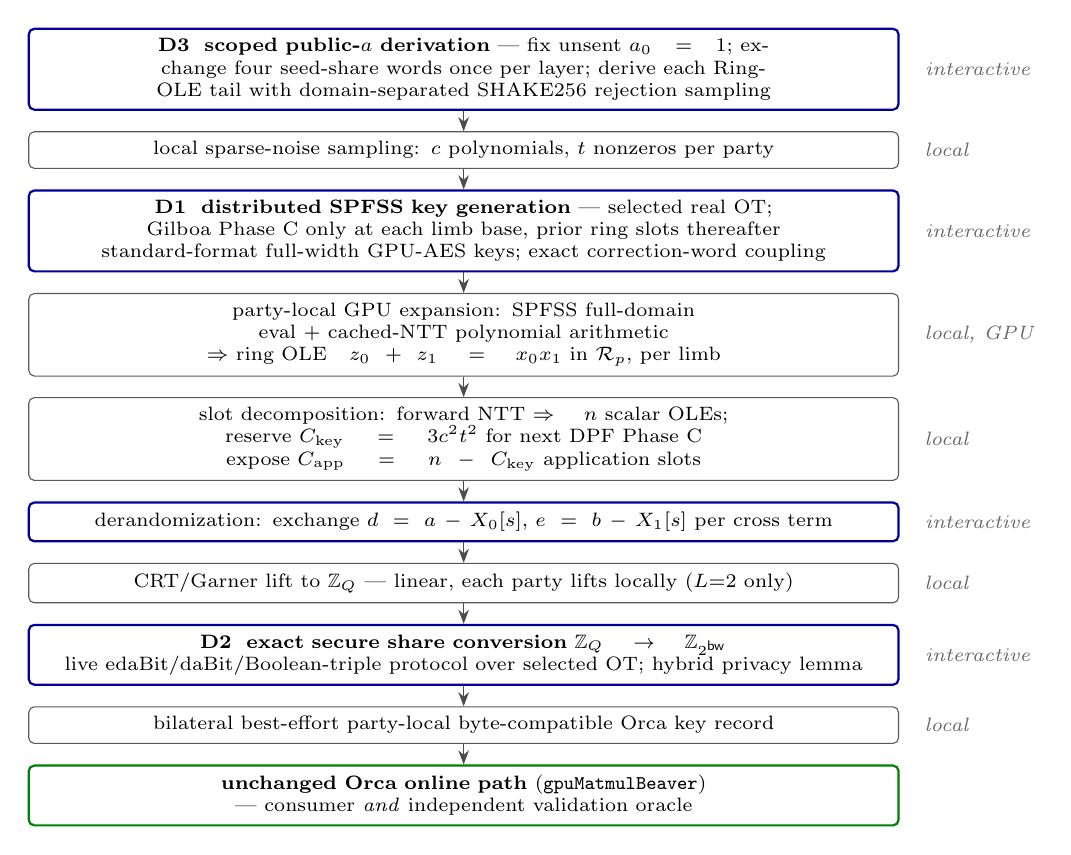
\begin{tikzpicture}[
  node distance=2.6mm,
  st/.style={draw, rounded corners=2pt, align=center, font=\scriptsize,
             inner sep=3.5pt, text width=108mm},
  loc/.style={st, draw=black!65},
  int/.style={st, draw=blue!60!black, thick},
  ora/.style={st, draw=red!70!black, thick, dashed},
  fin/.style={st, draw=green!50!black, thick},
  tag/.style={font=\scriptsize\itshape, text=black!60, anchor=west},
  arr/.style={-{Stealth[length=1.8mm]}, black!70}
]
\node[int] (coin) {\textbf{D3\ \ scoped public-$a$ derivation} --- fix unsent $a_0=1$; exchange four seed-share words once per layer; derive each Ring-OLE tail with domain-separated SHAKE256 rejection sampling};
\node[loc, below=of coin] (noise) {local sparse-noise sampling: $c$ polynomials, $t$ nonzeros per party};
\node[int, below=of noise] (kg) {\textbf{D1\ \ distributed SPFSS key generation} --- selected real OT; Gilboa Phase C only at each limb base, prior ring slots thereafter\\ standard-format full-width GPU-AES keys; exact correction-word coupling};
\node[loc, below=of kg] (exp) {party-local GPU expansion: SPFSS full-domain eval $+$ cached-NTT polynomial arithmetic\\ $\Rightarrow$ ring OLE\quad $z_0+z_1 = x_0x_1$ in $\Ring_p$, per limb};
\node[loc, below=of exp] (slot) {slot decomposition: forward NTT $\Rightarrow n$ scalar OLEs; reserve $C_{\rm key}=3c^2t^2$ for next DPF Phase C\\ expose $C_{\rm app}=n-C_{\rm key}$ application slots};
\node[int, below=of slot] (der) {derandomization: exchange $d = a - X_0[s]$,\ $e = b - X_1[s]$ per cross term};
\node[loc, below=of der] (crt) {CRT/Garner lift to $\Z_\Q$ --- linear, each party lifts locally ($L{=}2$ only)};
\node[int, below=of crt] (conv) {\textbf{D2\ \ exact secure share conversion} $\Z_\Q \to \modtwo$\\ live edaBit/daBit/Boolean-triple protocol over selected OT; hybrid privacy lemma};
\node[loc, below=of conv] (wr) {bilateral best-effort party-local byte-compatible Orca key record};
\node[fin, below=of wr] (onl) {\textbf{unchanged Orca online path} (\texttt{gpuMatmulBeaver}) --- consumer \emph{and} independent validation oracle};
\foreach \a/\b in {coin/noise, noise/kg, kg/exp, exp/slot, slot/der, der/crt, crt/conv, conv/wr, wr/onl}
  \draw[arr] (\a) -- (\b);
\node[tag, right=2mm of coin.east] {interactive};
\node[tag, right=2mm of noise.east] {local};
\node[tag, right=2mm of kg.east] {interactive};
\node[tag, right=2mm of exp.east] {local, GPU};
\node[tag, right=2mm of slot.east] {local};
\node[tag, right=2mm of der.east] {interactive};
\node[tag, right=2mm of crt.east] {local};
\node[tag, right=2mm of conv.east] {interactive};
\node[tag, right=2mm of wr.east] {local};
\end{tikzpicture}
\caption{Live forward-linear pipeline. Both parties run as independent
processes on distinct GPUs. Blue-framed stages exchange messages over same-host
TCP after mutual HMAC-SHA256 endpoint/context establishment; later protocol
bytes have no per-message integrity. Other stages are party-local, and
Ring-LPN expansion runs on the GPU. The unchanged online consumer runs only in
the post-exit checker.}
\label{fig:pipeline}
\end{figure}

\subsection{Setting and threat model}
\label{sec:threat}

Two computationally bounded parties; \textbf{static semi-honest}
(honest-but-curious) corruption of one party. The conditional theorem assumes
authenticated point-to-point channels, AES as a PRG/PRF
($\lambda{=}128$), standard semi-honest security of the selected OT backend,
the Gilboa field-multiplication wrapper, and BGI DPF, plus decisional
splittable Ring-LPN for the exact selected sparse-noise distribution
(\S\ref{sec:design-params}). The canonical and classifier suites instantiate
SCI/IKNP. The separate EMP-Silent correctness/accounting rerun remains opt-in
and independently unreviewed. Current measurements use same-host loopback after
a mutual HMAC-SHA256 endpoint/context handshake, but later local protocol bytes
have no application-layer integrity. They are implementation/correctness
evidence for the conditional theorem rather than an authenticated-channel
deployment.

Out of scope: malicious security, external packet attackers, timing and
microarchitectural side channels, stateful training transitions, and
dealerless nonlinear DCF preprocessing. ``Dealerless Orca'' without the
forward-linear/FC qualifier is not claimable.

\paragraph{Current evidence boundary.} The host artifact of
\S\ref{sec:m1proto} remains a counted ideal-functionality prototype using the
noncryptographic splitmix64 correctness PRG.
The live path separately uses full-width GPU AES, the selected real OT backend,
epoch-zero Gilboa OLE, consume-once Ring-OLE-output bootstrap, a four-word
joint public seed, domain-separated SHAKE256 public-polynomial derivation, and
separate process/GPU state. The canonical and classifier suites use SCI/IKNP.
The separate current EMP-Silent route supplies focused correctness and
accounting evidence only; it remains independently unreviewed. The proof models
SHAKE256 as a public random oracle and remains
conditional on the unpinned Ring-LPN assumption; measured local traffic is not
an authenticated deployment. Therefore neither backend artifact establishes
an end-to-end 128-bit-security claim.

\subsection{D1: Distributed SPFSS key generation (removes G1)}
\label{sec:design-keygen}

\paragraph{What must be computed.} For each pair $(k,l)$ of noise nonzeros,
the parties must generate DPF keys for the point function with position
$\alpha = \mathrm{pos}^0_k + \mathrm{pos}^1_l$ (a value in $[0, 2n)$: products
of degree-$<n$ polynomials have unreduced degree up to $2n-2$; the negacyclic
fold $u[i] - u[i+n]$ is linear and applied locally after expansion) and
payload $\beta = \mathrm{val}^0_k \cdot \mathrm{val}^1_l \in \Z_p$. Observe
that the required sharing is \emph{already present in the problem}: $\alpha$
is additively shared (each party knows its own summand) and $\beta$ is
multiplicatively shared, with no extra protocol.

\paragraph{Protocol.} We adopt the Doerner--shelat two-party DPF key
generation~\cite{doerner2017floram} in the variant used by the PCG
literature~\cite{boyle2019efficient,boyle2020ringlpn}. The parties walk the
GGM tree level by level. Off the secret path the two parties' nodes are
identical, so XORing each party's aggregate PRG expansions leaves the on-path
contribution needed for that level's correction word. Selection by the
current secret-shared bit of $\alpha$ uses a 1-of-2 OT on
$\lambda$-bit strings. We keep control/tag bits separate from the full
$\lambda$-bit seed state, following the formal BGI
construction~\cite{boyle2016fss}. We do not derive tags from seed LSBs: the
S1 target carries 128 secret seed bits and separate tags.

For the arithmetic payload, let $A_b$ be party $b$'s signed leaf-seed
aggregate and $F_b$ its signed control-bit aggregate. A first scalar OLE
produces $\gamma_0+\gamma_1=\beta_0\beta_1=\beta$. Set
\[
d_0=\gamma_0-A_0,\quad d_1=\gamma_1-A_1,\qquad
s_0=F_0,\quad s_1=F_1,
\]
so $d_0+d_1=\beta-A_0-A_1$ and
$s_0+s_1=F_0+F_1\in\{+1,-1\}$. Two additional directional OLEs share
$d_0s_1$ and $s_0d_1$; adding those cross-term shares to the local products
$d_0s_0$ and $d_1s_1$ yields shares
$w_0+w_1=(d_0+d_1)(s_0+s_1)$. The parties open only this standard public
key material, $\mathit{finalCW}=w_0+w_1$; they never open the $d_b$, $s_b$,
or their sign. The predecessor transcript opened both $F_b$ values. Although
their sign is marginally independent of $\alpha$, conditioning on one
party's leaf control-bit vector makes it select the class containing
$\alpha$, so that opening was invalid.

The input bits of $\alpha$ come from a secure ripple adder
($\log(2n)-1$ Beaver bit triples). This is the concrete integration choice
for arithmetic position shares, not a claim of new ripple-adder research.
The known 1-OT-per-level walk remains an unimplemented performance
optimization.

\paragraph{Prototype status (implemented; \S\ref{sec:m1proto}).} The
party-separated host implementation generates standard-format DPF keys from
shared $(\alpha,\beta)$ and passes full-domain validation by the
\emph{unchanged} existing evaluator on every tree tested: 2{,}432 key pairs,
both CRT primes, depths through $\log(2n)=14$. It uses ideal-functionality
OT, bit triples, and three scalar OLEs, plus the evaluator's non-cryptographic
correctness PRG; these are exactly why the executable is not evidence of
computational privacy. At depth 14 it records 28 string OTs, 13 bit triples,
3 scalar OLEs, 1{,}908 logical opened bits, and 3{,}816 meaningful share bits
per tree. Neither bit count is measured transport traffic. The old-sign
regression reconstructs the removed sign only in the omniscient harness and
confirms that it selects a proper leaf-control-bit class containing the true
point; this is a regression model of the old leak, not a privacy proof.

A real-transport path runs the same protocol as two OS processes over SCI/IKNP
and Gilboa OLE: 369/369 host-reference keys pass the unchanged evaluator;
88 full-width-AES keys pass batched and per-tree GPU evaluation. The exact
coupling lemma below proves that its correction words equal conditioned
standard DPF generation, so functional equality is no longer substituted for
distribution equality. Single-key privacy still invokes the standard DPF/PRG
theorem; this component result does not establish Ring-LPN security.

\subsection{S1 security contract for D1 and FC composition}
\label{sec:s1contract}

\paragraph{Two-level ideal functionality, freshness, and state topology.}
The numeric $\mathit{sid}$ remains a compatibility/session handle.  The actual
global base invocation is a public nonzero 128-bit $\mathit{iid}$.  For every
primitive the parties use the fixed-width big-endian tuple
\[
(\mathsf{v},\mathit{iid},\mathit{layerID},\mathit{kind},\mathit{layer},
\mathit{direction},\mathit{limb},\mathit{ringBatch},\mathit{tree},
\mathit{phase},\mathit{ordinal},\mathit{convChunk},\mathit{outputSlot}),
\]
with $2^{64}-1$ in every nonapplicable unsigned coordinate, and hash the
domain-prefixed encoding with SHA-256.  The encoding is injective before
hashing.  Hash collision resistance is an explicit assumption.
Here $\mathit{layerID}$ hashes only the stable operator, shape, arithmetic,
Ring-LPN parameters, and layer ordinal; it excludes $\mathit{iid}$,
compatibility SID, ledger, deployment channel, and OT backend.
Before OT setup or private-DRBG construction, both parties validate the exact
finite range plan and consume $\mathit{iid}$ in owner-only append-only ledgers:
no-replace create, write/fsync, atomic rename, and directory fsync.  A
duplicate, retry/restart, collision, malformed/truncated or crash-left pending
entry aborts before publication; consumed attempts never roll back and unused
tail slots are discarded.  Both version-3 party records carry $\mathit{iid}$
and the digest binding it to the layer and plan.  This additionally assumes a
trusted local filesystem with the stated durability and no adversarial storage
rollback. All publication attempts in one administrative deployment must use
this same persistent namespace; replacing it with a fresh, copied, or
rolled-back root is an explicit excluded deployment behavior.

For a public $(\mathit{iid},\mathit{cid},\mathit{tree},\dpfd,p)$,
$\mathcal F_{\mathrm{DDPF}}$ receives
$(\mathit{off}_b,\beta_b,\mathit{root}_b)$ from $P_b$, where
$0\leq\mathit{off}_b<2^{\dpfd-1}$, $\beta_b\in\Z_p^*$ is canonically
encoded, and $\mathit{root}_b$ is that party's uniform 128-bit random-tape
draw. It rejects a malformed, unclaimed, or duplicate identifier with the same
public abort at both parties before consuming correlation. Otherwise it sets
$\alpha=\mathit{off}_0+\mathit{off}_1$ without modular wrap and
$\beta=\beta_0\beta_1\bmod p$, runs standard DPF generation conditioned on
the supplied roots, and returns only $K_b$ to $P_b$. A batch may contain
arbitrarily correlated or repeated private inputs, but every tree uses a
distinct identifier, independent roots, and fresh primitive correlation.

The stateful $\mathcal F_{\mathrm{FC}}$ takes a public ordered topology table
whose entries reference public mask-wire handles. A handle names one
$\Z_{2^\bw}$ mask and its additive shares; repeated handles intentionally
reuse those shares. A training-layer row names
$(X,W,Y_{\rm bias},V_W,V_Y,G)$, its public truncation/optimizer parameters,
and whether momentum is enabled; current \texttt{FCLayer} requires bias.
Each matrix product creates a fresh product-output handle $R_C$ (source-level
\texttt{mask\_Z}) and splits
\[
 C_0+C_1=AB+R_C \pmod {2^\bw}.
\]
Forward reads $(X,W)$ and emits
$X_b\Vert W_b\Vert C_{\mathrm f,b}$; weight gradient reads the same $X$ plus
the incoming gradient handle $G$ and emits
$G_b\Vert C_{\mathrm{dW},b}$; input gradient, when enabled, reads that same
$G$ and the same $W$ and emits only $C_{\mathrm{dX},b}$.

The source-level forward transition broadcasts and adds persistent
$Y_{\rm bias}$ to $R_{C,\mathrm f}$ before truncation; the truncated result is
the next activation-mask handle. Backward row-sums $G$ to obtain the bias
gradient $dY$, truncates the $dX$ output, and applies both optimizer
transitions
$(W,V_W,dW)\mapsto(W',V_W')$ and
$(Y_{\rm bias},V_Y,dY)\mapsto(Y_{\rm bias}',V_Y')$.
Current Orca initializes $W,Y_{\rm bias},V_W,V_Y$ to zero; $X$ comes from the
preceding truncated output. These persistent operand/state masks are neither
resampled nor assumed independent per invocation. Every OT/DPF/OLE/conversion
correlation remains fresh even when a public mask handle is reused.
The live artifact implements and checks one complete forward FC matmul.
Bias/truncation, backward $dW/dX$, bias-gradient, and optimizer state
transitions require a new stateful extension before any training-layer claim.

All ideal calls carry the complete tuple above.  DPF Phase A triples, Phase B
directional string OTs, Phase C scalar OLEs, public-polynomial coefficients,
derandomization openings, conversion daBits/edaBits/Boolean triples, and used
output slots occupy disjoint coordinates.  The transport backend is not a
coordinate, so switching IKNP/silent implementations cannot authorize reuse.
Repeated operand-mask values remain legal only under distinct correlation IDs.
$\mathcal F_{\mathrm{BT}}$ returns private XOR shares of fresh uniform
$(a,b,c=a\wedge b)$; the Beaver openings remain real protocol messages.
$\mathcal F_{\mathrm{OT}}^{128}$ reveals only the selected sender string, and
$\mathcal F_{\mathrm{OLE}}^p$ samples $g_0$ uniformly and sets
$g_1=x_0x_1-g_0$. The composition additionally names these boundaries.
$\mathcal F_{\mathrm{BMUL}}^p$ instead consumes a registered Ring-OLE slot
with $Z_0+Z_1=X_0X_1$, reveals $\Delta_b=u_b-X_b$, and returns
$g_0=Z_0+\Delta_1X_0+\Delta_0\Delta_1$ and
$g_1=Z_1+\Delta_0X_1$. These output shares retain their exact correlation
with the registered slot; they are not fresh-share
$\mathcal F_{\mathrm{OLE}}^p$ outputs.
$\mathcal F_{\mathrm{PUBA}}^{p,H}$ exchanges one uniform 256-bit seed share
from each party per layer and XORs them into one joint seed. For each fresh
Ring-OLE scope it fixes the unsent identity $a_0=1$ and rejection-samples the
tail from the exact V2 byte query $\mathsf Q$ defined in
\S\ref{sec:design-seeds}. Distinct full scope/parameter queries define
independent exact-uniform $a_1,\ldots,a_{c-1}$ in the random-oracle model.
$\mathcal F_{\mathrm{RINGOLE}}^{\chi,b}$ is role-indexed and conditioned on
the corrupt party's complete local expansion state. It reruns the source-local
expansion to preserve both
$X_b=e_{b,0}+\sum_{i=1}^{c-1}a_i e_{b,i}$ and the recomputable $Z_b$, samples
only hidden $X_{1-b}$ uniformly, and sets
$Z_{1-b}=X_bX_{1-b}-Z_b$. Thus neither corrupt output is resampled.
$\mathcal F_{\mathrm{CONV}}$ handles canonical CRT shares. For canonical
$z_b\in[0,Q)$, this functionality computes
\[
 S=z_0+z_1,\quad \mathit{wrap}=[S\ge Q],\quad
 v=S-\mathit{wrap}\,Q,
\]
then returns uniform additive shares of $v\bmod 2^\bw$ and never opens
$\mathit{wrap}$. The live composition realizes these interfaces over the
selected real OT backend and validates its finalized keys only after both party
processes exit.

For canonical additive shares,
$a_0+a_1<2^{\bw+1}$ and $b_0+b_1<2^{\bw+1}$, so a length-$K$
integer dot product is strictly below $K\,2^{2\bw+2}$. The FC functionality
accepts only public triples satisfying $K\,2^{2\bw+2}<Q$: reduction modulo
$2^\bw$ then gives the intended mask product before any reduction modulo $Q$.
This rules out q62/bw32 entirely, caps q62/bw24 at
$K\leq2^{12}-1$, and is checked before masks are read; q62/bw32
inadmissibility is independently exercised by the executable negative
control in \texttt{test\_orca\_zp\_bridge}; the live FC path enforces the same
public bound before private-mask sampling and never performs a clear
value-dependent test. The deployed Ring-LPN GPU expansion uses four
domain-separated AES calls per node: plaintexts 0 and 2 produce full 128-bit
child seeds, while plaintexts 1 and 3 produce separate control bits.
Host/device parity and 88 two-process GPU-evaluated keys are gated. The
centralized benchmark kernel still derives roots from one 64-bit
\texttt{seed\_base} and is not security evidence. The live path instead uses
OpenSSL-private-DRBG roots/noise/masks and fixes the unsent identity $a_0=1$.
It exchanges four seed-share words once per layer and derives every
per-instance $(c-1)n$ tail through domain-separated SHAKE256 rejection
sampling. This is exact in the stated random-oracle hybrid, not a
standard-model public-coin construction. The exact key-distribution coupling
and conversion simulator close the remaining algebraic hybrid obligations.
Concrete Ring-LPN security parameters and an authenticated deployment remain
open; no end-to-end 128-bit claim is made.

\paragraph{Leakage and abort contract.}
Common leakage consists of protocol/session and party-role identifiers; the
parameter set, $L,\dpfd,p,n,c,t$, CRT limbs, noise mode, epoch and batch/tree
counts; public layer shapes, layouts, invocation kind, wire-handle topology,
slot/access order, serialized field lengths, fixed message lengths and
dependency schedule; common DPF correction words and
$\mathit{finalCW}$; masked openings
$\epsilon,\delta,d,e$ and the specified conversion openings; both exchanged
256-bit public-seed shares, their XOR joint seed, and the public Ring-LPN
vectors derived from it; and the common accept/abort stage.
$P_b$ additionally sees only its own DPF inputs/root draw, retained mask
shares, local frontier/noise/output-mask state, sender/receiver
OT view, triple/OLE shares, authenticated messages, output DPF keys, and
emitted Orca fields. The other inputs, roots, keys, mask shares, hidden
leaf-control sign, conversion wrap, unused OT messages, OLE masks, and PCG
state remain hidden. Public mask-handle reuse is required topology; reuse of
primitive correlation or private random-tape draws is prohibited. External
packet observers, timing/microarchitectural side channels, active security,
fairness, and availability remain out of scope.

\paragraph{Exact D1 hybrid transcript.}
The proof target is the
$(\mathcal F_{\mathrm{BT}},\mathcal F_{\mathrm{OT}}^{128},
\mathcal F_{\mathrm{PHASEC}}^p)$-hybrid protocol instantiated by the current
source, where each Phase-C product uses fresh-share
$\mathcal F_{\mathrm{OLE}}^p$ at a limb's base epoch or consume-once stateful
$\mathcal F_{\mathrm{BMUL}}^p$ thereafter. \emph{Phase A}: for each of the
$\dpfd-1$ carry positions, obtain one fresh bit triple, reveal both parties'
shares of the two masked one-bit
values $(\epsilon_j,\delta_j)$, apply the Beaver equation, and update
XOR-shared carry and point bits. This exposes $2(\dpfd-1)$ logical bits as
$4(\dpfd-1)$ transmitted shares. The private position summands are the
Ring-LPN noise positions, so uniform-mode sums are triangular; regular-mode
offsets give the corresponding public-bucket shift, not a uniform modular
point.

\emph{Phase B}: at level $i$, each party locally expands its live seeds,
XOR-aggregates left/right seed and flag children, and defines
$Z_b=S_b^{\mathrm L}\oplus S_b^{\mathrm R}$. Two directional 128-bit OTs
share $a_i(Z_0\oplus Z_1)$. Parties reveal their shares of the standard
seed correction word and two flag correction words, then advance locally.
These are exactly $130\dpfd$ logical opened bits and $260\dpfd$ meaningful
share bits.

\emph{Phase C}: one OLE shares
$\gamma_0+\gamma_1=\beta_0\beta_1$. With
$d_b=\gamma_b-A_b$ and $s_b=F_b$, two directional OLEs share
$d_0s_1$ and $s_0d_1$. Each party sets
$w_b=d_bs_b+x_b+y_b$ and reveals only $w_b$, giving the standard
$\mathit{finalCW}=w_0+w_1$. Neither $d_b$, $s_b$, nor
$s_0+s_1$ is opened. Thus
\[
\begin{aligned}
\text{logical opened bits}&=2(\dpfd-1)+130\dpfd+\lceil\log_2 p\rceil,\\
\text{meaningful share bits}&=4(\dpfd-1)+260\dpfd+
 2\lceil\log_2 p\rceil .
\end{aligned}
\]

\emph{Concrete post-base realization}: a reserved prior Ring-OLE slot gives
$(X_b,Z_b)$ with $Z_0+Z_1=X_0X_1$. For any Phase-C product
$u_0u_1$, the parties exchange $\Delta_b=u_b-X_b$ and output
\[
g_0=Z_0+\Delta_1X_0+\Delta_0\Delta_1,\qquad
g_1=Z_1+\Delta_0X_1.
\]
Their sum is $u_0u_1$. In the role-conditioned ideal Ring-OLE boundary the
honest $X_{1-b}$ is uniform, hence the received $\Delta_{1-b}$ is a one-time
pad independent of the honest input. The simulator samples that difference
uniformly and computes the corrupt output with the same role-specific equation
and retained $(X_b,Z_b)$ state. This exactly realizes
$\mathcal F_{\mathrm{BMUL}}^p$; it does not claim a fresh-uniform OLE output
share. Distinct consume-once slot identifiers compose sequentially. The
abstract counts
above remain the standalone DPF contract. A bootstrapped tree concretely opens
six masked field elements plus \textit{finalCW}, recorded as
$7\lceil\log_2p\rceil$ logical and $8\lceil\log_2p\rceil$ transmitted-share-
width bits in Phase C.

\paragraph{Exact coupling to standard DPF generation.}
After any fixed common-CW prefix, pair the parties' states at each tree prefix.
The standard invariant gives equal seed/tag states off the path of $\alpha$
and opposite tags at its prefix, so all off-path values cancel from the joint
XOR aggregates. With $a=a_0\oplus a_1$ and
$Z_b=S_b^{\mathrm L}\oplus S_b^{\mathrm R}$, substituting the two selected OT
outputs into the opened seed-CW shares gives
\[
\mathit{sCW}=
S_0^{\mathrm R}\oplus S_1^{\mathrm R}\oplus
a(Z_0\oplus Z_1)
=
\begin{cases}
S_0^{\mathrm R}\oplus S_1^{\mathrm R},&a=0,\\
S_0^{\mathrm L}\oplus S_1^{\mathrm L},&a=1.
\end{cases}
\]
This is exactly the standard losing-branch seed correction. The flag words are
\[
\mathit{tLCW}=T_0^{\mathrm L}\oplus T_1^{\mathrm L}\oplus a\oplus1,
\qquad
\mathit{tRCW}=T_0^{\mathrm R}\oplus T_1^{\mathrm R}\oplus a,
\]
so induction preserves the invariant and matches every standard correction
word. At the leaves cancellation gives
$A=A_0+A_1=\operatorname{convert}(s_{0,\alpha})-\operatorname{convert}(s_{1,\alpha})$ and
$F=F_0+F_1=t_{0,\alpha}-t_{1,\alpha}\in\{+1,-1\}$. Phase C reconstructs
\[
\mathit{finalCW}=(\beta-A)F,
\]
which is $\beta-A$ for tags $(1,0)$ and $A-\beta$ for $(0,1)$, exactly the
standard final correction. Thus, conditioned on the supplied roots, both
output keys equal standard generation deterministically; independent uniform
roots give the same joint distribution. This algebraic coupling is separate
from the standard single-key privacy theorem and its PRG assumption.

\paragraph{D1 batch-simulation lemma at the ideal boundary.}
Fix either corrupt party, its complete arbitrarily correlated input/root
vector, public order and identifiers, and its full ideal output-key vector.
Condition each key on the same root supplied by that party. The following
algorithms generate the complete hybrid view with the real conditional
distribution. The exact coupling above identifies those conditioned outputs
with standard DPF generation; concrete PRG/transport security is separate.

\emph{Corrupt $P_0$.}
For each tree, take the root seed and common correction words from $K_0$ and
expand the local frontier. At every carry, sample $P_0$'s three bit-triple
shares, compute its actual sent shares of $(\delta_j,\epsilon_j)$, sample the
two reconstructed openings uniformly, and set the honest sent shares to the
XOR complements. Apply $P_0$'s real Beaver equation, including the public
$\delta_j\epsilon_j$ term, and the carry recurrence. Hidden honest triple
shares one-time-pad both openings, so induction from carry zero gives the
exact joint carry/point-share view.

At every level, derive $P_0$'s aggregates. In the first OT it is receiver:
sample the selected output, uniform under the honest sender's fresh mask. In
the second it is sender: sample $r_0$ and record
$(r_0,r_0\oplus Z_0)$. Compute its seed/flag opening shares with the real
equations and set the honest shares to complements of the words fixed by
$K_0$. Use the following source branch for each of the three Phase-C products.
For a declared product with output $\rho$ and inputs $(u_0^\rho,u_1^\rho)$,
at a limb's base epoch sample the corrupt
$\mathcal F_{\mathrm{OLE}}^p$ output $\rho_0$ uniformly. At a later epoch,
take that product's retained slot $(X_0^\rho,Z_0^\rho)$, set
$\Delta_0^\rho=u_0^\rho-X_0^\rho$, sample only the honest masked difference
$\Delta_1^\rho$ uniformly, and compute
\[
\rho_0=Z_0^\rho+\Delta_1^\rho X_0^\rho+
\Delta_0^\rho\Delta_1^\rho .
\]
Apply this branch first to
$(u_0^\gamma,u_1^\gamma)=(\beta_0,\beta_1)$, then set
$d_0=\gamma_0-A_0$ and $s_0=F_0$. Apply it next to
$(u_0^x,u_1^x)=(d_0,s_1)$ and
$(u_0^y,u_1^y)=(s_0,d_1)$. Thus $(\gamma_0,x_0,y_0)$ need not be independent
or uniform after the base epoch. Compute $w_0=d_0s_0+x_0+y_0$ and emit only
$w_1=\mathit{finalCW}-w_0$. This ordering also covers zero intermediate
values and preserves the complete retained-state correlation; it does not
infer the hidden sign.

\emph{Corrupt $P_1$.}
Take the root and common words from $K_1$. Sample its triple shares and
masked openings as above, but apply $P_1$'s Beaver equation without the
public $\delta_j\epsilon_j$ term. At each level record its first-OT sender
pair $(r_1,r_1\oplus Z_1)$ and sample its selected second-OT receiver output;
derive its own seed/flag shares and complement to the fixed common words.
Use the same source branch for each declared product. At a limb's base epoch,
sample the corrupt $\mathcal F_{\mathrm{OLE}}^p$ output $\rho_1$ uniformly.
At a later epoch, take that product's retained $(X_1^\rho,Z_1^\rho)$, set
$\Delta_1^\rho=u_1^\rho-X_1^\rho$, sample only the honest masked difference
$\Delta_0^\rho$ uniformly, and compute
\[
\rho_1=Z_1^\rho+\Delta_0^\rho X_1^\rho .
\]
Apply this branch first to
$(u_0^\gamma,u_1^\gamma)=(\beta_0,\beta_1)$, then set
$d_1=\gamma_1-A_1$ and $s_1=F_1$. Apply it next to
$(u_0^x,u_1^x)=(d_0,s_1)$ and
$(u_0^y,u_1^y)=(s_0,d_1)$. Thus $(\gamma_1,x_1,y_1)$ need not be independent
or uniform after the base epoch. Compute $w_1=d_1s_1+x_1+y_1$ and emit only
$w_0=\mathit{finalCW}-w_1$, preserving the complete retained-state
correlation.

Both simulators enforce a consumed-correlation-ID ledger before every ideal
call and proceed tree by tree conditioned on the complete prior state.
Therefore repeated/correlated private summands do not invalidate the
one-time-pad hybrids. S1 treats local coins as independent consumed
random-tape draws and makes the root explicit; S3 must prove a concrete,
state-consistent CSPRNG interface. In the end-to-end hybrid, only the honest
party's hidden PRG stream may be replaced by ideal random strings; the corrupt
party's stream and retained state remain consistent.

\begin{table}[ht]
\centering
\scriptsize
\begin{tabular}{>{\raggedright\arraybackslash}p{0.12\linewidth}>{\raggedright\arraybackslash}p{0.58\linewidth}>{\raggedright\arraybackslash}p{0.18\linewidth}}
\toprule
ID & Proof obligation & Current status\\
\midrule
P-CORR & Keys reconstruct $\beta[x=\alpha]$. & 2{,}432/2{,}432 executable passes\\
P-DIST & Couple correction words to standard DPF generation conditioned on
both roots. & exact algebraic coupling above\\
P-KEY & One standard key hides point/payload. & standard DPF/PRG theorem;
concrete reduction review open\\
P-POS & Prove the exact uniform/regular Ring-LPN exponent distribution. &
contract fixed; distribution/reduction audit open\\
P-ADD & Simulate either ripple-adder view with explicit triple/opening
equations. & closed in bit-triple hybrid\\
P-LEVEL & Simulate both OT roles and CW shares conditioned on each full key. &
closed in OT hybrid\\
P-PAYLOAD & Simulate the three-OLE view without the removed sign, including
zero intermediates. & closed in OLE hybrid\\
P-BATCH/P-FRESH & Preserve correlated tree inputs and reject correlation-ID
reuse before output. & D1 lemma + persistent invocation/ledger controls\\
P-RNG/P-PCG & Realize private tapes/exact public $a$ and prove Ring-LPN OLE at
the selected distribution. & RNG implemented; PCG reduction/parameters open\\
P-CONV & Realize exact modulo-$Q$ conversion without revealing wrap. &
closed in the edaBit/daBit/triple hybrid; transport assumptions explicit\\
P-TOPO/P-PROC & Match stateful reuse/serialization and two-process execution. &
forward FC and classifier evidence closed on SCI/IKNP; training state and
authenticated deployment open\\
\bottomrule
\end{tabular}
\caption{S1 proof contract. Closed rows are hybrid-transcript lemmas only,
not a computational-security claim; open rows are binding later-stage gates.}
\label{tab:s1proof}
\end{table}

\paragraph{Conditional forward-FC theorem.}
Let $\chi_{\mathrm U}$ sample exactly $t$ distinct positions without
replacement and $\chi_{\mathrm R}$ sample one position in each of $t$ public
equal buckets; in both cases coefficients are independent uniform elements of
$\Z_p^*$. Assume decisional module-Ring-LPN for the exact selected distribution:
for independent uniform $a_1,\ldots,a_{c-1}\in R=\Z_p[X]/(X^n+1)$ and
$e_0,\ldots,e_{c-1}\leftarrow\chi$,
\[
 (a_1,\ldots,a_{c-1},e_0+\sum_{i=1}^{c-1}a_i e_i)
\]
is indistinguishable from replacing the final component by uniform $R$.
Sampling all $c$ public entries would be a different, unreviewed assumption.
Also model SHAKE256 on the exact V2 byte query $\mathsf Q$ of
\S\ref{sec:design-seeds} as the public random oracle used for independently
scoped public-$a$ vectors, and assume the four-call GPU AES expansion is a PRG,
the standard BGI single-key theorem, semi-honest security of the selected OT
backend and Gilboa field-multiplication wrapper, authenticated channels, and
the BCG+20 Figure-2 reduction.

Under those assumptions, the live forward protocol realizes the forward-matmul
restriction of $\mathcal F_{\mathrm{FC}}$ with the leakage above. The simulator
samples one joint 256-bit public seed, sets the honest four-word XOR share
against the corrupt share, and programs every fresh exact $\mathsf Q$ query
with an independent uniform stream. It retains the corrupt random tape,
local $e_b$, and D1 key, reruns the source-local expansion, and thereby
preserves both
$X_b=e_{b,0}+\sum_{i=1}^{c-1}a_i e_{b,i}$ and recomputable $Z_b$. It then
replaces the first limb instance's external transports by ideal OLE and applies
the complete D1 simulator and standard-key coupling; replaces only hidden
$X_{1-b}$ and sets $Z_{1-b}=X_bX_{1-b}-Z_b$; then registers that ideal
output's reserved suffix with $\mathcal F_{\mathrm{BMUL}}^p$. For the next DPF,
it samples each honest masked difference uniformly and derives the corrupt
Phase-C output from the retained slot exactly. The generalized D1 simulator and
Figure-2 replacement then provide the next ideal Ring-OLE state. Induction in
public epoch order covers every later DPF and
expansion without assuming its own output. It samples each opposing application
derandomization opening under the corresponding fresh hidden OLE share, applies
the exact conversion simulator, and adds the fresh uniform output-mask share
before serializing $A_b\Vert B_b\Vert C_b$. Every replacement conditions on
prior state. Across $m$ fresh direction/limb/batch instances, the hybrid incurs
at most the sum of the $m$ role-indexed Figure-2/module-Ring-LPN advantages; it
does not infer a joint claim from one unconditioned single-instance sample.
This theorem excludes the measured post-handshake TCP transport, which has no
per-message integrity, as well as malicious parties and unimplemented training
state transitions. The source execution uses $(n,c,t)=(8192,2,8)$; the separate
full-graph control overrides $n=262144$ at the same $(c,t)$. Both are feasibility
configurations with no concrete-security claim.

\paragraph{Bootstrapping (and why it is not circular).} Key generation
consumes three scalar OLEs per DPF tree; expansion produces $n$ slot OLEs per
ring OLE. The factory therefore feeds itself precisely when
\begin{equation}
3c^2 t^2 \;<\; n,
\label{eq:bootstrap}
\end{equation}
The live protocol realizes these epochs. It exposes the prefix
$C_{\rm app}=n-C_{\rm key}$ of every Ring-OLE output to FC and reserves the
final suffix
$C_{\rm key}=3c^2t^2$ for the next DPF; it rejects $C_{\rm key}\ge n$ before OT
setup. The first instance of each CRT limb uses a fixed external batch of
Gilboa multiplications. In public $(\textit{ring batch},\textit{direction},
\textit{limb})$ order, every later instance consumes the preceding output's
reserved suffix using the stateful masked-difference realization above. The final
per-limb continuation reserve is discarded with the consume-once invocation.
At $(c,t,n)=(2,8,8192)$, $C_{\rm key}=768$,
$C_{\rm app}=7424$, and the output/input surplus is
$8192/768=10.67\times$.

Noncircularity is an induction: epoch zero first replaces external OLE by
$\mathcal F_{\rm OLE}$, then DPF by $\mathcal F_{\rm DDPF}$ and expansion by
the role-indexed ideal Ring-OLE. Its reserved suffix registers state for
$\mathcal F_{\rm BMUL}$, whose exact role-specific simulator supplies the next
DPF's Phase-C view without replacing the correlated output by fresh
$\mathcal F_{\rm OLE}$ shares. Repeat the DPF and Figure-2 replacements in
public order. Distinct slot IDs compose sequentially. The conclusion remains
conditional on the multi-instance Ring-LPN obligation; bootstrapping does not
solve that open assumption.

For the classifier run, the exact count is
$2L\lceil MKN/C_{\rm app}\rceil=276$ Ring-OLE instances
($L=2$, 69 batches). Per party, 1{,}536 Phase-C products come from epoch zero,
210{,}432 come from PCG output, and the 211{,}968 reserved slots split exactly
into 210{,}432 consumed plus 1{,}536 terminal-discarded slots; 1{,}024
application slots are also unused and reported. If $t=64$ at $n=8192$, then
$3c^2t^2=49{,}152>8{,}192$ and the executable capacity control rejects before
output; a reviewed parameter set must increase $n$.


\paragraph{GPU batching.} All trees of a generation batch advance
level-synchronously: the depth-14 tree walk has 14 sequential batched
AES/PRG expansions and OT selections, independent of tree count. One CUDA
block now owns each tree's XOR and final modular reductions; warp/block
reductions replace the former same-address leaf atomics without changing the
DPF transcript. The secure ripple adder, correction-word openings, and
two-stage payload multiplication add dependency stages. The TCP implementation
reports semantic dependency layers separately from direction switches; neither
counter is a packet/network-round measurement.

\paragraph{Cost model (per ring-OLE limb).} Each DPF tree of depth $d$ costs
$\lambda d$ correlated-OT instances; Ferret-class silent OT estimates place
each instance at roughly 1--8 bits of real traffic across maturity regimes.
The live implementation instead measures its selected backend; this range is
analytic context only. With uniform noise there are
$c^2t^2$ trees of depth $\log(2n) = 14$. With \emph{regular} noise (one
nonzero per width-$n/t$ bucket), the $t^2$ product points of each polynomial
pair fall on $2t-1$ predictable diagonals, so the same $c^2t^2$ trees shrink
to depth $\log(2n/t)$, grouped as $c^2(2t-1)$ SPFSS instances over the smaller
domain.\footnote{The 2026-06-10 draft priced the regular-noise row per SPFSS
\emph{instance} ($c^2(2t-1)$ units of depth 14), giving 107{,}520 OT
instances at $t{=}8$; the counts below are per DPF \emph{tree}, matching
\texttt{build\_spfss\_keys()}, and supersede it. Separate $t{=}64$
diagnostics record 881\,ms and 9.04\,MB for uniform noise and 61\,ms and
5.53\,MB for regular noise. The distributions and SPFSS domains differ, so no
timing or key-size ratio is claimed.}

\begin{table}[ht]
\centering
\small
\begin{tabular}{lrrrrr}
\toprule
noise, $t$ ($c{=}2$) & DPF trees & depth & OT instances & scalar OLEs & est.\ silent-OT comm.\\
\midrule
uniform, $t{=}8$  & 256    & 14 & 458{,}752   & 768    & 0.06--0.46\,MB\\
regular, $t{=}8$  & 256    & 11 & 360{,}448   & 768    & 0.05--0.36\,MB\\
uniform, $t{=}64$ & 16{,}384 & 14 & 29{,}360{,}128 & 49{,}152 & 3.7--29\,MB\\
regular, $t{=}64$ & 16{,}384 & 8  & 16{,}777{,}216 & 49{,}152 & 2.1--17\,MB\\
\bottomrule
\end{tabular}
\caption{Distributed key-generation cost per ring-OLE limb (derived).
$n=8192$, $\lambda=128$; depth is $\log_2(2n)$ resp.\
$\log_2(2n/t)$. Scalar OLEs equal three times the tree count. The silent-OT
communication column is an analytic range, not the live byte counter. The live
implementation measures its selected backend and pays the scalar-OLE OT cost
only for the first instance of each CRT limb; later rows consume Ring-LPN
output slots and exchange the counted masked field words. The standalone host
prototype of \S\ref{sec:m1proto} retains 2 string OTs per level,
depth$-1$ bit triples, and three ideal scalar OLEs per tree.}
\label{tab:keygen}
\end{table}

\subsection{D2: PCG-sourced share conversion (removes G2)}
\label{sec:design-convert}

\paragraph{The problem.} The pipeline holds additive shares over $\Z_\Q$
(prime world, where NTTs exist); Orca needs shares over $\modtwo$ (hardware
world, where they do not). Reducing both shares mod $2^{\bw}$ is wrong
whenever the integer share-sum wrapped past $\Q$ --- and that \emph{wrap bit}
depends on both shares jointly, so computing it requires an actual secure
protocol.

\paragraph{The protocol (validated two-process artifact).} For canonical
$z_b\in[0,\Q)$, let $S=z_0+z_1<2\Q$ and
$\ell=\lceil\log_2 2\Q\rceil$ ($\ell{=}63$ at q64, $125$ at q128).
The edaBit functionality samples uniform $R\in\Z_{2^\ell}$, an independent
uniform arithmetic first share, and independent uniform XOR masks for its
bits; the daBit functionality analogously shares one random bit over
$\Z_2$ and $\Z_{2^\bw}$. The live artifact realizes one exact daBit with one
128-bit OT, composes one exact edaBit from $\ell$ daBits (the coefficient-one
arithmetic share makes the sum uniform), and realizes each Boolean triple
with two one-bit OTs. Under fresh correlations: (1)~mask and open
$A=(z_0+z_1+R)\bmod 2^\ell$; (2)~a ripple adder recovers Boolean shares of
$S=A-R$; (3)~a second adder obtains
$w=[S\ge\Q]$ from the carry of $S+(2^\ell-\Q)$; (4)~the daBit converts $w$
to arithmetic shares; and (5)~each party computes
$r_i=(z_i-\Q w_i)\bmod 2^\bw$. Thus
$r_0+r_1=((z_0+z_1)\bmod\Q)\bmod 2^\bw$ and $w$ is never opened.
\paragraph{Ideal-OT wrapper lemma.}
These custom correlations are exact constructions in the
$\mathcal F_{\mathrm{OT}}$ hybrid. For one daBit, $P_0$ samples bit $x$ and
arithmetic mask $r$, offers $(x-r,1-x-r)$ in $\Z_{2^\ell}$, and $P_1$ selects
with bit $y$. The arithmetic shares sum to $x\oplus y$, matching the local
Boolean shares; the unused message and choice remain hidden and either
arithmetic share is uniform. Weighting $\ell$ fresh daBits by $2^j$ gives the
edaBit arithmetic share
$R_b=\sum_{j=0}^{\ell-1}2^j d_{j,b}\bmod2^\ell$ and its matching XOR-shared
bits; freshness makes reconstructed $R$ uniform. For a Boolean triple, each
party samples local $a_b,b_b$ and a fresh sender mask, sends
$(m_b,m_b\oplus b_b)$ once, receives once with choice $a_b$, and XORs its
local product, sender mask, and receiver output. Expanding the two cross terms
gives $c_0\oplus c_1=(a_0\oplus a_1)\wedge(b_0\oplus b_1)$. For either
corruption the simulator retains the corrupt random tape and selected output
and chooses only the hidden mask/unused message; fresh identifiers give the
batched weighted-edaBit and triple composition used below.


Independent processes over TCP pass 76 conversions in each of four q64/q128
and bit-width configurations: exact boundary sums
$0,\Q-1,\Q,2\Q-2$, random inputs, forced wraps, and layer-shaped inner
products, with zero mismatches and a corrupted-output control. The ripple
circuit consumes $2(\ell-1)$ AND triples, $2\ell-1$ post-mask dependency
stages, $5\ell-3$ logical opened bits, and $10\ell-6$ meaningful share bits.
The last count excludes byte padding, framing, setup, and OT payloads; the
artifact separately measures setup, correlation, and online bytes and
direction switches. Dependency stages are semantic depth, not measured
network rounds.

\paragraph{Semi-honest privacy at the correlation boundary.}
$A$ is uniform because $R$ is uniform. Every ripple-AND opening is one-time
padded by a fresh Boolean triple, and the B2A opening is $w\oplus d$ for a
fresh uniform daBit $d$; hence these opened values are simulatable and reveal
neither $S$ nor $w$. The output-share distribution also matches the ideal
functionality: $\Q$ is odd, so multiplication by $\Q$ permutes
$\Z_{2^\bw}$; a uniform arithmetic daBit share makes each
$z_i-\Q w_i$ uniform subject to the required sum. Given an ideal local output,
the simulator solves uniquely for that local daBit share using
$\Q^{-1}\bmod2^\bw$, samples all local Boolean/edaBit/triple shares with their
real marginals, chooses every masked opening uniformly, and completes only the
honest transmitted shares. This closes P-CONV in the
$(\mathcal F_{\mathrm{edaBit}},\mathcal F_{\mathrm{daBit}},
\mathcal F_{\mathrm{BT}})$ hybrid. The concrete path remains conditional on
the selected backend's semi-honest OT security and an authenticated channel.

\paragraph{What remains for production D2.} Two things. \emph{Sourcing:} AND triples come
from a binary PCG (the $\Z_2$ instantiation of our own pipeline, or
expand-accumulate codes~\cite{couteau2021silver}; Ferret~\cite{yang2020ferret}
yields them at $\sim$1 bit amortized), edaBits from random bit-shares by the
standard construction~\cite{escudero2020edabits} ($O(\ell)$ AND triples each,
one-time batch), daBits from the same batch. \emph{Depth:} the ripple
comparator becomes a parallel-prefix (Rabbit-style~\cite{makri2021rabbit})
comparison --- carries obey an associative generate/propagate rule, so all of
them come out of a $O(\log\ell)$-depth tree. That depth bounds the eventual
interactive schedule, but actual network rounds must be measured after the
prefix circuit is implemented and batched.

\begin{table}[ht]
\centering
\small
\begin{tabular}{lrr}
\toprule
per $\modtwo$ output & q64 ($\ell{=}63$) & q128 ($\ell{=}125$)\\
\midrule
AND triples $=2(\ell{-}1)$ & 124 & 248\\
edaBit bits $=\ell$        & 63  & 125\\
daBits                     & 1   & 1\\
logical opened bits $=5\ell-3$ & 312 & 622\\
meaningful share bits $=10\ell-6$ & 624 & 1{,}244\\
post-mask dependency stages, ripple $=2\ell{-}1$ & 125 & 249\\
post-mask dependency stages, prefix target & $\sim$7 & $\sim$8\\
\bottomrule
\end{tabular}
\caption{Validated two-process conversion cost per output with executable
transcript accounting, plus the prefix-comparator dependency-depth target.
The earlier 375/747 column mixed the two shares of the masked-$A$ opening with
logical AND/B2A openings; it was not a coherent metric. ``Meaningful share
bits'' is the sum of protocol-defined share widths, not encoded traffic.
Measured byte and direction-switch columns are separate; a prefix comparator
changes correlation counts and must report its own split.}
\label{tab:convert}
\end{table}

\subsection{D3: Scoped public vectors and private randomness (removes G3)}
\label{sec:design-seeds}

The live protocol uses two distinct randomness classes. Private DPF roots,
masks, and sparse noise are drawn from each process's OpenSSL private DRBG.
For the Ring-LPN public vector, $a_0$ is exactly the identity polynomial and is
sampled and sent by neither party. Once per linear layer, each party exchanges
four uniform 64-bit seed-share words; both XOR the raw shares to obtain one
joint 256-bit public seed. The implemented random-oracle query is exactly
\[
\begin{split}
\mathsf Q={}&
\operatorname{ASCII}(\texttt{RINGLPN\_PUBLIC\_A\_V2})
\mathbin\Vert \texttt{0x00}\mathbin\Vert \mathit{seed}_{32}
\mathbin\Vert \mathit{scope\_id}_{32}\\
&{}\mathbin\Vert \operatorname{LE64}(n)
\mathbin\Vert \operatorname{LE64}(c)
\mathbin\Vert \operatorname{LE64}(t)
\mathbin\Vert \operatorname{LE64}(\mathit{log\_domain})
\mathbin\Vert \operatorname{LE64}(\mathit{direction})\\
&{}\mathbin\Vert \operatorname{LE64}(\mathit{limb})
\mathbin\Vert \operatorname{LE64}(\mathit{slot\_batch})
\mathbin\Vert \operatorname{LE64}(\mathit{modulus})
\mathbin\Vert \operatorname{LE64}(\mathit{regular})
\mathbin\Vert \operatorname{LE64}(\mathit{chunk}).
\end{split}
\]
The ASCII domain plus its explicit terminal byte is 20 bytes;
$\mathit{seed}_{32}$ and the full $\mathit{scope\_id}_{32}$ are raw 32-byte
values, and each remaining field is an unsigned 64-bit little-endian word in the displayed
order, with $\mathit{regular}\in\{0,1\}$. SHAKE256 streams on $\mathsf Q$ are
rejection-sampled into $\Z_p$ to
derive the $(c-1)n$-coefficient tail. Distinct full scope/parameter/chunk
queries give independent exact-uniform vectors in the random-oracle model.
For q128, both limb queries reuse the same joint seed; the encoded
$\mathit{limb}$ and $\mathit{modulus}$ fields domain-separate them.

The short public seed cannot provide information-theoretic full-vector entropy;
the real implementation therefore instantiates an explicit SHAKE256
random-oracle assumption. This removes the former multi-gigabyte public-tail
exchange without silently reusing one public vector or pretending the
construction is exact in the standard model. A malicious extension would
replace the fixed-order semi-honest seed exchange with commit/open.

\subsection{D4: Two-process deployment and endpoint/context establishment}
\label{sec:design-deploy}

The composed artifact runs the parties as two OS processes on distinct GPUs
over two SCI-style TCP channels. Before preflight, each direction performs a
versioned mutual HMAC-SHA256 challenge/response binding role, direction,
invocation ID, claim digest, and fresh nonces. This rejects a rogue connector,
replay, reflection, wrong role/context, or wrong shared secret at connection
establishment; it does not MAC or encrypt later protocol bytes. Each process
reads only its own sampled noise and emits only its own key record. The post-exit
checker reads both records, reconstructs the clear masks only for validation,
and invokes unchanged
\texttt{readGPUMatmulKey}/\texttt{gpuMatmulBeaver}. The runner rejects
mismatched preflight manifests, stale output, malformed or swapped records,
and unilateral publication, and removes raw party records after validation.

Measured application traffic includes DPF Phase-A/B OT payloads, epoch-zero
Gilboa OLE payloads, four public-seed words per party and layer, cross-term
derandomization openings, conversion correlation and online messages, and
final synchronization. It excludes selected-backend base-OT setup and TCP/IP
overhead. Total recorded transport includes the separately counted 43{,}658
base-OT setup bytes. An unexecuted two-host launcher tunnels the streams over
pinned SSH; current retained rows are same-host loopback and do not establish
authenticated protocol-channel integrity or host isolation.

\subsection{D5: Security parameter audit (G4 remains open)}
\label{sec:design-params}

The assumption behind step 1 of \S\ref{sec:motivation-pcg} is
\textbf{reducible module-Ring-LPN} over each deployed prime-field limb:
$(a_1,\ldots,a_{c-1},e_0+\sum_{i=1}^{c-1}a_i e_i)$ is pseudorandom for
regular sparse secrets $e_i$. The public vector is exactly
$a=(1,a_1,\ldots,a_{c-1})$; the former all-uniform-$c$ construction is not the
BCG+20/component distribution and carries no reviewed assumption here.
The q128 path is two prime-field instances whose public vectors are
independently domain-separated outputs from one shared joint seed in the
SHAKE256 random-oracle model, followed by CRT; it is not one instance over a
124-bit field, and its limbs are not independently seeded.
The splitting of $X^n+1$ buys slot packing but exposes reductions modulo
sparse low-degree factors. This is the BCG+20 reducible-ring setting, not
directly the quasi-abelian group-algebra setting of
Bombar et al.~\cite{bombar2023quasiabelian}.

Parameter names matter: BCG+20's total weight is $w=ct$, so its Table-1 row
$(c,w)=(4,64)$ maps to this implementation's per-polynomial $t=16$, not
$t=64$. The corrected full version does not provide one reproducible
projection rule: Section~8.2 derives
$c d(1-(1-1/d)^t)$, whereas Section~9.1 uses
$w-cd+(c(d-1)+w)(1-1/d)^{t-1}$; its literal smallest-factor test selects
degree 16 for this row, while Table~1 reports degree 128.

A source audit also invalidated several preliminary estimator outputs. The
accepted EUROCRYPT 2024 aggregate calls attack formulas containing
$\binom{N-k}{t'}$ and $\binom{N-k-1}{t'}$, so a projected tuple must at least
satisfy $t'\le N-k-1=d-1$. The artifact silently evaluates out-of-range
combinations. Thus the recorded 57.293-bit $(c,t,d)=(4,16,16)$, 218.641-bit
$(4,64,64)$, and 257.023-bit $(4,34,64)$ values are invalid function calls,
not attack costs. Mechanically defined rows include 135.12 bits at
$(4,16,64)$, BCG's degree-128 row at 145.85 bits, and 190.53 bits at
$(2,128,256)$, but these remain hypothetical finite-field regular-noise model
outputs rather than Ring-LPN security estimates.

The exact regular-projection law remains pinned as a finite combinatorial
statement: $t$ independently occupied source positions map into $d$ buckets,
with the corresponding occupancy distribution and independent uniform
nonzero coefficients in $\mathbb F_p^*$ conditioned on projected support.
It covers collisions and cancellation. It is freshly source-bound to live
\texttt{two\_party\_spfss.h} SHA-256 prefix \texttt{fbdb56f8}: a semantic diff
from the prior audited revision changes only optional Phase-C OLE-source
forwarding in the CPU baseline; \texttt{validate\_party\_noise} and
\texttt{sample\_party\_noise} are unchanged. This establishes current
distribution correspondence, not a security pin.

The source-pinned 2024 regular-ISD calculator and exact automorphism-orbit law
remain model diagnostics. The self-tested 2025 hybrid-RSD formula artifact was
freshly regenerated: its script/CSV SHA-256 prefixes are
\texttt{cbcedaf6}/\texttt{1f671d94}, with the script digest embedded in every
row. Its 20 rows are not an attack implementation, quantum cost, or
structured-code reduction, and no reviewed newer-attack instantiation maps
these diagnostics to the live tuple.
Therefore D5 has not pinned $n,c,t,p_0,p_1$, and this proposal makes no
128-bit classical or quantum claim. The measured $n=2^{17},c=4,t=34$
implementation NO-GO remains valid independently: regular noise requires
$t\mid n$, and the uniform layout would materialize 7{,}272{,}923{,}136 host
slots (at least 123.6\,GB in one process). No replacement parameter is pinned.

\subsection{Composition status}
\label{sec:design-composition}
\begin{table}[ht]
\centering
\small
\begin{tabular}{>{\raggedright\arraybackslash}p{2.6cm}>{\raggedright\arraybackslash}p{2.1cm}>{\raggedright\arraybackslash}p{5.3cm}>{\raggedright\arraybackslash}p{2.7cm}}
\toprule
boundary & status & executable/proof evidence & consequence\\
\midrule
G1 centralized keygen & closed for forward FC & live distributed GPU-AES DPF
keys in six cases and the model run; exact correction-word coupling &
no centralized key generator; trusted-dealer-free only in stated RO model\\
G2 share conversion & closed in hybrid & live selected-OT conversion plus
exact simulator; wrap remains hidden & conditional semi-honest privacy\\
G3 shared/private RNG & closed in RO hybrid & per-party OpenSSL DRBG, unsent
identity $a_0=1$, four-word joint seed, and independently scoped SHAKE256
rejection sampling & exact required distribution in the stated random-oracle
model\\
process/state separation & executable; peer isolation open & distinct
processes, GPUs, input files, and output records, but the current loopback
runner uses one UID; a fail-closed two-host isolation harness exists but has
not been executed & functional composition only, not an OS isolation claim\\
G4 concrete parameters & \textbf{open} & source audit rejects prior pins; no
reviewed replacement & no security-level claim\\
G5 graph/state and broader scope & known-zero composition closed; setup open &
trusted nonlinear adapter plus the complete stock graph and terminal
reconstruction & nonlinear setup and private or trained models remain open\\
\bottomrule
\end{tabular}
\caption{Current composition status. ``Closed'' is scoped to each row's stated
boundary: the theorem is forward-linear, and graph closure is one known-zero
control. Deployment still requires distinct hosts, authenticated transport,
and a reviewed Ring-LPN parameter pin.}
\label{tab:composition}
\end{table}

\subsection{Per-layer cost model (worked example)}
\label{sec:design-cost}

For one FC layer $(M,K,N)$ at $L$ limbs, the current self-sustaining artifact
uses
\[
2L\left\lceil\frac{MKN}{C_{\rm app}}\right\rceil
\]
Ring OLEs. Application derandomization sends $4MKNL$ field words. Every
Ring-OLE instance after the first per limb also consumes $C_{\rm key}$ earlier
slots and sends two masked-difference field words per consumed slot. Conversions
equal $MN$ (each per Table~\ref{tab:convert}); key-generation material per Ring
OLE is in Table~\ref{tab:keygen}. The online phase is unchanged because keys
are byte-compatible.

Worked executable example, $16{\times}32{\times}16$ at q64 ($L{=}1$,
$\bw{=}16$, $n{=}8192,c{=}2,t{=}8$): $MKN=8192$ cross terms per direction
need four Ring OLEs at $C_{\rm app}=7424$. They provide 29{,}696 application
slots, use 16{,}384, and report 13{,}312 unused. Of 3{,}072 reserved slots,
2{,}304 bootstrap the three post-base instances and 768 are terminally
discarded. Application derandomization sends 32{,}768 field words; bootstrap
adds 4{,}608 masked-difference field words. The $MN=256$ conversions use
31{,}744 AND triples plus 256 daBits. These capacities and consume/discard
equalities are executable CSV gates, not a projected production epoch.

\section{Experiment setup}
\label{sec:experiments}

\subsection{Platform and environment}
\label{sec:platform}

All measurements in this document were produced on one host: $4\times$ NVIDIA
RTX 5000 Ada (32{,}760\,MiB each, compute capability 8.9; driver 560.35.03),
CUDA 12.6, Linux 6.8, and a 32-core CPU allocation. Builds run on the host.
Two-party tests run as separate processes pinned to distinct GPUs through
\texttt{CUDA\_VISIBLE\_DEVICES} over single-host IPv4 loopback. The canonical
q64/q128 and classifier suites use SCI/IKNP. A separate current EMP-Silent
five-case/16-control rerun is opt-in and independently unreviewed. Both
backends use \texttt{PartyChannel}/SCI \texttt{NetIO}; local measurements
authenticate endpoint/context before preflight but do not protect later bytes
at the application layer. Application-byte counters exclude backend setup and
TCP/IP overhead.
The GPU NTT backend is a
cheddar-derived merged-stage kernel family (signed Montgomery arithmetic;
q32/q64/q128-CRT; negacyclic) with the Hadamard product adaptively fused into
the inverse-NTT load and forward NTTs of fixed public vectors cached across
expansion iterations.

\subsection{Validation methodology}
\label{sec:methodology}

Three rules, applied to every artifact. (1)~\emph{Independent oracles}: fast
implementations are validated against separately written references --- the
GPU NTT against a host reference (\texttt{host\_polymul\_reference}), the
generator's internals against host suites (135/57/36 host validation cases),
the end-to-end pipeline against Orca's \emph{unchanged} online code
reconstructing the correct product. (2)~\emph{Party-separation discipline}:
transcript artifacts compute each party's view in separated state; any read
across the boundary is an explicitly named oracle. (3)~\emph{Mechanical
gates}: every artifact ships source + build script + run script + CSV/MD/log;
suites exit non-zero on failure. The canonical checkpoint revalidates all host
and GPU component gates:
\begin{center}
{\small\verb+RUN_GPU_SMOKE=1 REQUIRE_GPU_SMOKE=1 PATH=/usr/local/cuda/bin:$PATH \+}\\
{\small\verb+  scripts/run_paper_checkpoint_smoke.sh+}
\end{center}
and must print \texttt{ALL GATES PASS}. The exact-shape repeated evaluation is
separately regenerated by \texttt{scripts/run\_two\_party\_fc\_model\_scale.sh}.

\paragraph{Pinned reproduction boundary.}
\texttt{scripts/Dockerfile.reproduction} contains no source or credentials and
binds the CUDA base digest, dated Ubuntu snapshot, exact package set, GPU
architecture, and TeX toolchain. A clean recursive clone is mounted at runtime;
\path{scripts/reproduce_publication.sh} rejects dirty source, missing or
untracked checkpoint evidence, checksum drift, root-owned outputs, stale
destinations, a nonconforming GPU, any gate mutation outside regenerable
result paths, and any surviving private key, state, ledger, or scratch
artifact. The shared FC/Conv binary approval binds two byte-identical builds
whose command, working-directory, and build-environment receipts use only
canonical clone, source, and build-root tokens; a self-consistently rehashed
receipt with a raw workstation path is rejected before record execution. Its
\texttt{local-smoke} mode rebuilds this PDF and the full canonical gate but
ends with an explicit ``not two-host publication evidence'' marker. Publication
mode additionally requires an owner-authorized annotated source tag, an
operator-supplied tag/commit consistency object whose shape and self-digest are
checked (no cryptographic signer is verified), an immutable runtime image and
in-image binary identity, pinned SSH host identity, a separate owner-only
persistent read-write ledger mount, and the authenticated two-host/checker
manifests. Those release and deployment identities have not
been issued; this remains an internal reproducibility contract rather than
released two-host evidence.

\subsection{Verified artifacts and matched baseline}
\label{sec:baseline}

\paragraph{Single-process real-generator diagnostic.} The older
suite\footnote{Artifact \texttt{bench\_orca\_fc\_real\_ole\_transcript}; per-case
results in Table~\ref{tab:suite}'s source CSV.} validates the Ring-LPN engine
and slot/Orca algebra in nine q64/q128 uniform/regular cases. It uses
centralized DPF key generation and clear exact conversion at explicitly named
O1/O2 boundaries. Its narrow stage timings are diagnostic only and are not
compared with the live end-to-end measurements.

\begin{table}[ht]
\centering
\small
\begin{tabular}{lrrrrr}
\toprule
case & ring OLEs & ideal-OLE equiv. & slots used & opened $\Z_p$ words & contract\\
\midrule
q64, $16{\times}32{\times}16$, $\bw{=}16$ & 2 & 16{,}384 & 8{,}192 & 32{,}768 & pass\\
q128, $16{\times}16{\times}16$, $\bw{=}32$ & 4 & 8{,}192 & 4{,}096 & 32{,}768 & pass\\
\bottomrule
\end{tabular}
\caption{Representative rows of the single-process diagnostic
(\texttt{orca\_fc\_real\_ole\_\allowbreak transcript\_\allowbreak
transcript\_\allowbreak suite.csv}). ``Ideal-OLE equiv.''\ is the number of
per-scalar OLE calls the same layer consumed before slot packing.}
\label{tab:suite}
\end{table}

\paragraph{Distributed key-generation protocol-logic prototype
(corrected and rerun 2026-08-06).}
\label{sec:m1proto}
The artifact\footnote{\texttt{test\_distributed\_dpf\_keygen}; per-case
results in \texttt{distributed\_dpf\_keygen\_prototype.csv}.} implements the
two-party key-generation protocol of \S\ref{sec:design-keygen}
party-separated on the host. Cross-party values flow only through counted
ideal functionalities (1-of-2 string OT, Beaver bit triples, and three
scalar OLEs) or explicit openings. It emits the standard existing
\texttt{spfss\_host::DPFKey} format, consumed by the untouched
\texttt{spfss\_host::dpfEvalAll}. That evaluator uses a splitmix64
correctness PRG explicitly labelled non-cryptographic; the artifact is
therefore a protocol-logic and compatibility prototype, not a secure/private
implementation.

The suite (Table~\ref{tab:m1proto}) generates 2{,}432 key pairs across six
configurations, tree depths 4--14, and both CRT primes. Every pair
full-domain-evaluates to $\beta\cdot[x{=}\alpha]$. In every configuration,
the first two trees deterministically cover $\alpha=0$ and
$\alpha=2^{\dpfd}-2$, factors $1$ and $p-1$, and resulting payloads $p-1$ and
$1$; the remaining trees use random nonzero payload factors. Eight centralized
references pass through the same evaluator; five independent root-seed,
seed-CW, left-flag-CW, right-flag-CW, and final-CW corruptions fail; and six invalid point/payload encodings abort
before correlation is consumed. The field
\texttt{old\_sign\_opening\_leak\_control=yes} records that the omniscient
regression model reconstructed the removed sign and observed a proper
party-0 leaf-control-bit class containing the true point. This demonstrates
the old transcript's distinguishing power; it is not a privacy proof.
Every row also requires ideal-mask-draw accounting and a duplicate-correlation-ID
negative control to pass. The gate is wired into the repository's one-command
re-validation (\S\ref{sec:methodology}).

\begin{table}[ht]
\centering
\small
{\scriptsize
\setlength{\tabcolsep}{3pt}
\begin{tabular}{lrrrrrrrr}
\toprule
prime & depth & trees & pass & string OTs & triples & OLEs & logical open & meaningful share bits\\
\midrule
$p_0$ & 4  & 512 & 512/512 & 8  & 3  & 3 & 588   & 1{,}176\\
$p_0$ & 8  & 512 & 512/512 & 16 & 7  & 3 & 1{,}116 & 2{,}232\\
$p_0$ & 11 & 384 & 384/384 & 22 & 10 & 3 & 1{,}512 & 3{,}024\\
$p_0$ & 14 & 256 & 256/256 & 28 & 13 & 3 & 1{,}908 & 3{,}816\\
$p_1$ & 14 & 256 & 256/256 & 28 & 13 & 3 & 1{,}908 & 3{,}816\\
$p_1$ & 8  & 512 & 512/512 & 16 & 7  & 3 & 1{,}116 & 2{,}232\\
\bottomrule
\end{tabular}
}
\caption{Distributed DPF key-generation host results.}
\label{tab:m1proto}
\end{table}

Source: \texttt{distributed\_\allowbreak dpf\_\allowbreak
keygen\_\allowbreak prototype.csv}. For tree depth $\dpfd$, per-tree counts
match $2\dpfd$ string OTs,
$\dpfd-1$ bit triples, three scalar OLEs,
$2(\dpfd-1)+130\dpfd+\lceil\log_2 p\rceil$ logical opened bits, and
$4(\dpfd-1)+260\dpfd+2\lceil\log_2 p\rceil$ meaningful share bits. Every row
reports \texttt{transcript\_accounting=pass},
\texttt{ideal\_mask\_draw\_\allowbreak accounting=pass}, and
\texttt{correlation\_reuse\_\allowbreak control=pass}. Timings are approximately
2.0\,ms per depth-14 tree, single-threaded and including validation; they are
run observations, not transport measurements. Table~\ref{tab:m1proto} proves
functional compatibility, edge correctness, and ideal-primitive accounting,
not computational privacy or 128-bit security.

\paragraph{Retained classifier-layer result (2026-08-10).}
The recorded artifact evaluates the exact inference classifier-layer shape
$1{\times}512{\times}1000$ at $\bw=32$ with
$(n,c,t)=(8192,2,8)$, q128, regular noise, $C_{\rm key}=768$, and
$C_{\rm app}=7424$. It executes 69 batches and 276 Ring-OLE instances.
The source implements GPU-batched distributed DPF generation with GPU-AES
expansion, tree-block correction-word/leaf reductions, and Ring-OLE-output
Phase-C bootstrap. Each process reads only its own private noise record, runs
on its own GPU, and emits only its own final key record. A 128-bit invocation
identifier and persistent consume-once correlation ledger reject replay,
duplicate, stale-tail, and stale-bootstrap use. After both processes exit, the
checker reconstructs the records, verifies the clear product, and invokes
unchanged \texttt{readGPUMatmulKey}/\texttt{gpuMatmulBeaver}.

Ten measured trials followed one warmup using the default SCI/IKNP backend.
The environment binds current binary SHA-256 \texttt{02eaaac9\ldots}. These
same-host timing/traffic rows authenticate endpoint roles and invocation
context before preflight, but later protocol bytes have no per-message
integrity. The public-vector construction exchanges four 64-bit seed-share
words per party and layer, then derives a fresh domain-separated SHAKE256 tail
per Ring-OLE while
treating $a_0=1$ as public without sending it. The aggregate CSV and
digest-bound metadata pass execution, record, transcript, freshness,
bootstrap-accounting, and unchanged-online checks; this table remains a
classifier-layer measurement, not full-model execution.

\begin{table}[ht]
\centering
\small
\begin{tabular}{@{}l r@{}}
\toprule
metric & current measured value\\
\midrule
warmup / measured trials & 1 / 10\\
mean setup-included critical path / sample SD & $4.011203588$ s / $0.036601967373448$ s\\
95\% Student-$t$ CI for mean & $[3.985020117867291,4.037387058132709]$ s\\
setup-included critical-path R-7 IQR & $0.03481908225$ s\\
median setup-included critical path & $4.0193924415$ s\\
median setup-included preprocessing/dealer ratio & $268.6769431352700\times$\\
median shape-matched \texttt{gpuKeygenMatmul} & $14.73535$ ms\\
median unchanged two-share online & $1.14969$ ms\\
application bytes, both directions & $182{,}372{,}344$\\
total recorded transport & $182{,}416{,}324$\\
public-$a$ 64-bit seed-share words, both parties & $8$\\
Phase-C products per party, epoch-zero / PCG & $1{,}536$ / $210{,}432$\\
reserved slots per party, consumed / terminal discard & $210{,}432$ / $1{,}536$\\
unused application slots per party & $1{,}024$\\
semantic protocol dependency layers & $11{,}023$\\
peak host / device-wide GPU-used bytes & $142{,}542{,}848$ / $31{,}929{,}597{,}952$\\
final payload bytes per party & $4{,}108{,}096$\\
serialized record bytes per party & $4{,}108{,}304$\\
\bottomrule
\end{tabular}
\caption{Exact retained ResNet18 classifier-layer result. Time statistics are over ten
measured trials; $268.6769431352700\times$ is the median of setup-included
shape-matched per-trial ratios, not the quotient of displayed medians.
Setup-included time is the per-layer sum of the party maximum of
\texttt{total\_us+preflight\_us+ot\_setup\_us}. It excludes
\texttt{PartyChannel} construction, socket establishment, and channel
authentication, so it is not true end-to-end time. GPU occupancy was
uncontrolled and the runs were not controlled on the same physical GPU, so
this is not a hardware-matched A/B comparison. The environment binds current
binary \texttt{02eaaac9\ldots}. Application bytes exclude selected-backend
base-OT
setup and TCP/IP overhead; total recorded transport includes 43{,}658 base-OT
setup bytes. The GPU-used value is a device-wide observation that includes
unrelated shared-GPU occupancy, not a process allocation measurement.}
\label{tab:modelscale}
\end{table}

\paragraph{Controlled CNN2/CNN3 FC matrix (2026-08-14).}
The source-authored workload manifest selects CNN2 FC4
($100{\times}256{\times}128$), CNN2 FC5
($100{\times}128{\times}10$), and CNN3 FC5
($100{\times}64{\times}10$). All use q128/bw32, regular noise, and the
feasibility tuple $(n,c,t)=(8192,2,8)$; they require 42, 18, and 9 Ring-LPN
batches, respectively. Every layer passes one warmup and ten measured trials,
for 30/30 passing measured layer trials. Both protocol parties run on distinct
quiescent RTX 5000 Ada GPUs. After they exit, the stock
\texttt{gpuKeygenMatmul} comparator runs on the quiescent physical GPU of the
sample's slower setup-included party; advisory per-GPU locks span the complete
run. Thus the comparator matches source shape, key contract, binary, allocator
and synchronization boundary, physical GPU, and observed quiescence. Execution
order is fixed as protocol then dealer, not randomized.

\begin{table}[ht]
\centering
\small
\begin{tabular}{@{}l rr@{}}
\toprule
metric & CNN2 all FC & CNN3 FC5\\
\midrule
FC layers / measured layer trials & $2$ / $20$ & $1$ / $10$\\
mean setup-included / sample SD (s) & $26.881842$ / $0.050965$ & $0.903894$ / $0.018971$\\
median / R-7 IQR (s) & $26.897711$ / $0.065754$ & $0.904910$ / $0.028512$\\
95\% Student-$t$ CI for mean (s) & $[26.845384,26.918301]$ & $[0.890323,0.917466]$\\
mean stock dealer / sample SD (ms) & $30.46697$ / $0.47174$ & $14.92146$ / $0.31011$\\
median stock dealer (ms) & $30.5729$ & $14.96295$\\
median paired setup-included ratio & $879.2970985824659\times$ & $60.3181599795375\times$\\
application / total transport bytes & $1{,}302{,}752{,}736$ / $1{,}302{,}840{,}696$ & $39{,}432{,}504$ / $39{,}476{,}484$\\
semantic dependency layers & $72{,}278$ & $1{,}663$\\
mean peak host RSS / process GPU bytes & $305{,}696{,}768$ / $431{,}095{,}808$ & $137{,}465{,}446$ / $431{,}095{,}808$\\
\bottomrule
\end{tabular}
\caption{Controlled model-FC feasibility matrix. CNN2 statistics sum both
retained FC layers within each measured model trial; CNN3 has one supported FC
layer. Setup-included time sums the per-layer critical-party
\texttt{total\_us+preflight\_us+ot\_setup\_us}; it still excludes channel
construction, socket establishment, authentication, checker time, and the
stock dealer. ``Semantic dependency layers'' are implementation schedule
depths, not packet or network-round counts. Total transport adds selected
SCI/IKNP base-OT setup bytes but excludes TCP/IP framing. The fixed
protocol-then-dealer order can retain order bias. All values are local
loopback feasibility measurements at unpinned parameters, not full-model,
WAN, security-level, or competitive-performance evidence.}
\label{tab:cnnmatrix}
\end{table}

In the retained classifier rows, legacy post-OT median Phase C is 0.041723\,s, Phase B is
1.955515\,s, Phase A is 0.2462935\,s, and GPU Ring-LPN expansion is
1.226650\,s.

\paragraph{Full-graph systems control.}
One retained source-bound q128/bw32 known-zero run consumes a fresh 21-record
ResNet18 convolution/FC set through the unchanged Orca linear consumers. Its
execution manifest overrides the source tuple from $(n,c,t)=(8192,2,8)$ to
$(262144,2,8)$ so the largest layers fit; this is an execution parameter, not a
security pin. The compiled graph contract is generated from, and hash-checked
against, the same source manifest used by the record-set gate. Its explicit
value-source registry binds every main and shortcut operand; the exact stock
forward order contains 21 linear calls, 21 stochastic truncations, 19 stock key
consumers (one MaxPool, 17 ReLUs, and classifier sign extension), 20 remask
edges, eight residual merges, integer GlobalAvgPool2D, and terminal
reconstruction.

The 21-record set contains 6{,}439 Ring-LPN batches, 25{,}756 Ring-OLE
instances, 6{,}593{,}536 DPF trees, and 130{,}774{,}336 final payload bytes per
party. In this one sequential run, the sum of legacy post-OT linear-layer
critical paths was 4{,}720.417\,s. The 50.161-s full-graph orchestrator wall
measurement covers the graph positive run and seven fail-closed graph-output
controls; it excludes record generation and is not positive-path end-to-end
latency. The record-consuming graph critical path was 11.852\,s. These
are not a timing distribution or competitive result.

A test-only trusted compatibility adapter reads both parties' source-bound
linear mask states, supplies both parties' truncation successor-mask shares
plus remask and terminal material, and emits the exact 62-item stock key stream,
including all nonlinear keys. It took 9.356\,s and produced
1{,}084{,}582{,}352 raw stock-key bytes per party. Each live party reads only
its own private linear, nonlinear, and persistent-state records. A separate
post-exit checker independently reconstructs every linear input/output, remask,
residual, pool, sign-extension, and terminal value from both published records
and rejects counter/order drift. Seven fail-closed
graph-output controls---forced second rename, reused invocation, stale output,
party-record swap, truncated nonlinear record, nonlinear payload corruption,
and digest-valid trace corruption---all reject without partial output;
source-manifest and topology mismatch controls also reject.

The retained 17-indexed-payload-file bundle plus \path{INDEX.json} at
\path{results/graph/resnet18_full_graph_checkpoint_2026_08_10/} excludes private
linear, mask-state, nonlinear, ledger, and output records. Its original
manifest-bound adapter provenance retains workstation/build-root strings, and
the historical linear assignment reused GPU 1 sequentially for party 1 and its
checker. These are non-secret internal/advisor metadata, but they block external
circulation and no longer satisfy the current retained-assignment policy. The
original bytes are preserved for transitive manifest/approval/INDEX integrity;
a fresh canonical three-GPU run with normalized provenance must replace this
checkpoint before release. The orchestration deliberately applied each
omniscient per-record correctness checker before feeding the same test record
to the graph control, so it does not evidence consume-once online deployment.
The trusted nonlinear key source means this is not dealerless nonlinear
preprocessing or added security evidence; known-zero inputs and weights mean it
is not private/trained inference, an accuracy result, deployment evidence, or a
full-model performance claim.

The closest in-artifact dealer comparator is stock
\texttt{gpuKeygenMatmul}, aligned on shape, masks, bit width,
allocator/synchronization boundary, and output bytes. The retained classifier
execution was not controlled on the same physical GPU and occupancy state, so
its $268.6769431352700\times$ statistic remains descriptive. The newer
CNN2/CNN3 matrix adds per-sample physical-GPU and quiescence control; its
$879.2970985824659\times$ and $60.3181599795375\times$ medians are controlled,
strongly negative stock-dealer comparisons rather than speedup claims.
A separately pinned stock libOTe Reverse-Cuckoo run and a project-prime
exact-$p_0$ native-folded adapter diagnostic are retained:
\begin{table}[ht]
\centering
\small
\begin{tabular}{@{}l r r r@{}}
\toprule
row & setup & online/full domain & protocol total\\
\midrule
stock Goldilocks & \multicolumn{3}{c}{12.43\,s process wall}\\
exact $p_0$ native-folded & 18.523424\,s & 2.116894\,s & 20.640318\,s\\
\bottomrule
\end{tabular}
\caption{Reverse-Cuckoo baselines at nominal $(n,c,t)=(2^{20},4,16)$.
The stock row uses internally sampled factors, synthetic preloaded base
correlations, CPU local sockets, Goldilocks arithmetic, and a 16-folded layout.
The exact-$p_0$ diagnostic uses 256 sets of 16 points (4,096 terms), checks
16,777,216 full-domain positions, and records 52,791,184 setup plus 1,425,584
online wire bytes. Its protocol total is 20.640318\,s and its
validation-inclusive total is 20.688314\,s.
Neither row is raw 31-diagonal GPU output, a function-matched
comparison, or a security-level result; no speedup ratio is reported.}
\label{tab:reverse-cuckoo}
\end{table}
\paragraph{Optional EMP-Silent feasibility rerun (2026-08-14).}
The current opt-in rerun binds FC binary \texttt{bf4e4f90\ldots}, authorized
bridge \texttt{435f3be6\ldots}, and EMP-OT revision
\texttt{2fca139f\ldots}. All five live cases and all sixteen rejection controls
pass; every declared directional 128-bit-OT inventory is consumed exactly.
\begin{table}[ht]
\centering
\small
\begin{tabular}{@{}l r r r r@{}}
\toprule
case & straight OTs & reversed OTs & $P_0$ sent & $P_1$ sent\\
\midrule
q64 regular small & 59{,}120 & 11{,}248 & 1{,}716{,}463 & 550{,}112\\
q64 uniform small & 62{,}192 & 14{,}320 & 1{,}766{,}383 & 600{,}032\\
q128 regular small & 118{,}232 & 22{,}496 & 2{,}645{,}481 & 739{,}129\\
q128 uniform small & 124{,}376 & 28{,}640 & 2{,}745{,}321 & 838{,}969\\
q64 regular multibatch & 93{,}184 & 37{,}376 & 2{,}159{,}029 & 739{,}717\\
\bottomrule
\end{tabular}
\caption{Focused EMP-Silent accounting. Byte columns sum instrumented backend
correlation, chosen-message adjustment, and ciphertext bytes sent; they exclude
channel authentication and TCP framing. The selected API exposes no
nonoverlapping base-OT subboundary. Inventories are equal at both parties.}
\label{tab:emp-silent}
\end{table}
There is one trial per case and all four GPUs carried unrelated resident
workloads. Timing/memory columns therefore support no comparison. The custom
SilentFerret revision remains independently unreviewed, so these rows make no
performance, bandwidth-improvement, security, or headline claim.

\paragraph{Performance anchors.}
Ring-OLE expansion ($n{=}8192$, $c{=}2$): 9.086\,ms (q64) and 18.230\,ms
(q128) for regular noise at the $t{=}8$ smoke point, one iteration per
configuration ($n{=}1$ each); separate $t{=}64$ diagnostics record 881\,ms
uniform and 61\,ms regular, with two timed iterations per mode ($n{=}2$ each;
four total), and pair-key bytes 9{,}044{,}160 (9.04\,MB) and 5{,}529{,}408
(5.53\,MB), respectively. The distributions and SPFSS domains differ, so no
ratio is claimed. SPFSS full-domain evaluation dominates
($\sim$99\%); the NTT is under 1\% ---
measured directly, and confirmed by the fact that a 2--8\% NTT-side
improvement left expansion time unchanged. The oracle-backed conversion stress
artifact is bit-exact on 8{,}516 conversions per configuration; the live
two-process OT-backed artifact passes 76 conversions in each of four
q64/q128/bit-width configurations, at the costs of
Table~\ref{tab:convert}. Byte-compatibility: with the integration flag off,
baseline Orca output is byte-identical (verified through the real two-party
FC test).

\subsection{Status gates and remaining experiments}
\label{sec:milestones}

\begin{description}
\item[Closed --- current live forward path.] The current focused two-process
  SCI/IKNP suite passes all five q64/q128 cases and controls, generating
  distributed GPU-AES DPF keys, self-bootstrapped Ring-LPN OLE shares, converted
  q32 masks, and byte-compatible Orca FC records. Every focused row records
  positive breadth-first call counts for both parties and zero root-to-leaf
  calls; all 21 shape plans pass. The current FC/Conv binaries begin
  \texttt{02eaaac9}/\texttt{975ac726}, and the focused approval digest begins
  \texttt{ce3cc3a5}. These are correctness/path-counter results, not current
  Conv0 timing or a breadth-first speedup claim. Sixteen negative
  controls cover endpoint/context authentication, replay, reflection, freshness,
  ledger integrity, nonpositive capacity, malformed/swapped records, and
  publication failure; the unchanged online consumer reconstructs the expected
  product.
\item[Closed narrowly --- model-FC matrix.] The source manifest selects CNN2
  FC4 and FC5 and CNN3 FC5; each passes one warmup and ten measured trials.
  Per-sample stock-dealer execution follows both parties on the quiescent
  physical GPU of the slower setup-included party. Aggregate median paired
  ratios are $879.2970985824659\times$ for CNN2 and
  $60.3181599795375\times$ for CNN3. This closes source coverage, repetition,
  dispersion, and same-hardware/quiescence control for these three FC layers,
  not competitive performance, parameter security, full-model execution, or
  network evaluation.
\item[Closed narrowly --- full-graph systems control.] One source-bound
  known-zero run binds a fresh 21-record set to all unchanged Conv2D/FC
  consumers, all secure truncations and stock nonlinear consumers, every
  projection/identity residual merge, GlobalAvgPool2D, sign extension, and
  terminal reconstruction. Manifest/topology, publication, nonlinear-record,
  and output-corruption controls reject. The trusted test-only adapter reads
  both mask states, supplies both truncation successor-mask shares plus
  remask/terminal material, and generates the nonlinear keys. Therefore
  dealerless nonlinear preprocessing remains open.
\item[Closed conditionally --- proof composition.] The theorem composes
  standard semi-honest DPF, OT/OLE, conversion, DRBG, and authenticated-channel
assumptions with a selected Ring-LPN sample distribution. The exact
regular-projection law is freshly bound to the current sampler, and the
self-tested hybrid-RSD formula evidence is freshly regenerated. The
structured-code hardness transfer, concrete parameter pin, and independent
cryptographic review remain open.
\item[Open --- parameters.] A reviewed structured-code and two-CRT-limb
  advantage analysis must pin $(n,c,t,p_0,p_1)$ before any security-level
  claim. All performance rows must then be rerun because the current point is
  feasibility-only.
\item[Open --- performance engineering.] Phase B remains the largest measured
  stage, followed by GPU Ring-LPN expansion and Phase A; Phase C is much
  smaller. Full-duplex Phase-A/B scheduling and retained asynchronous frontier
  allocation are complete. A source- and cost-audited specialized regular-DMPF
  design attempt returned NO-GO: no reviewed candidate preserved the fixed
  transcript, plain Ring-LPN boundary, application-slot budget, stock-key ABI,
  and deployed-shape cost simultaneously. Keep the measured DPF path for the
  approved full-linear systems integration and pursue algorithmic Phase-B/round
  reduction. The controlled model-FC matrix reports median setup-included
  shape-matched preprocessing/dealer ratios of $879.2970985824659\times$ for
  CNN2 and $60.3181599795375\times$ for CNN3. The result is not competitive;
  reruns at reviewed parameters and further Phase-B/dependency-layer work
  remain necessary.
\item[Open --- model realism and dealer scope.] Exact source-bound ResNet18
  graph coverage is closed for one known-zero input/weight control. It is not
  private or trained inference, accuracy evidence, a timing distribution, or
  full-model performance. Dealerless nonlinear key generation remains absent;
  repeated clean runs with private inputs and trained weights, including an
  accuracy-bearing evaluation, are still required before a broader systems
  claim.
\item[Open --- deployment.] Source contains fail-closed two-host coordination
  and peer-private container orchestration: both complete post-handshake
  streams are carried through one pinned-host-key, AEAD-only OpenSSH tunnel
  with bounded rekeying. No configured second host was available to execute it.
  Current evidence uses same-host loopback with authenticated endpoint/context
  establishment but no application-layer protection for later bytes; it cannot
  predict LAN/WAN latency, establish executed authenticated-channel integrity,
  or prove OS-level peer isolation.
\item[Open --- review.] A human cryptographer who did not author the artifact
  must review the DPF/OT/OLE/composition proof, the structured-code parameter
  argument, and the custom pinned EMP-Silent revision. Internal adversarial
  review and focused differential/correctness tests are not substitutes.
\item[Out of scope.] Training-state updates, a dealerless DCF-key protocol,
  active security, and full-model dealer removal require separate designs and
  evaluations.
\end{description}

\subsection{Reporting and claims discipline}
\label{sec:claims}

The current supported statement is: ``At unpinned feasibility parameters, a
live same-host two-process implementation generates party-local forward-linear
keys without a trusted dealer in the stated random-oracle model; those keys
match the stock Orca format and pass unchanged online computation. Endpoint
roles and invocation context are mutually HMAC-authenticated before preflight,
but later protocol bytes have no per-message integrity. A separate source-bound
known-zero control composes a fresh 21-record linear set with the exact stock
ResNet18 graph using a trusted test-only adapter that owns both truncation
successor-mask shares, remask/terminal material, and nonlinear keys. Conditional
semi-honest security applies only to the forward-linear theorem under its
explicit DPF, OT/OLE, authenticated-channel, and exact-distribution Ring-LPN
assumptions.''

The in-artifact quantitative dealer comparator is stock
\texttt{gpuKeygenMatmul}. The current CNN2/CNN3 matrix aligns source-authored
shapes, bit width, masks, output bytes, binary, allocator/synchronization
boundary, physical GPU, and observed quiescence for every sample. Its fixed
protocol-then-dealer order is not randomized, and its strongly negative ratios
remain local feasibility results. The older classifier rows lack physical-GPU
and occupancy control and remain descriptive only. The older single-process
Ring-OLE stage timers omit most live work and are not a baseline.
Prior dealerless PCG systems expose different correlations, parameter
assumptions, and applications; no compatible implementation has been measured
under this artifact's contract, so no cross-paper speedup ratio is reported.

Unsupported wording includes ``128-bit secure,'' ``faster than the dealer,''
``WAN-ready,'' ``dealerless full Orca,'' and any dealerless-nonlinear,
nonlinear-security, training-layer, private-inference, accuracy, or full-model
performance/security claim.
Every future performance table must identify topology, trust/oracle boundary,
coverage, exact parameters, counter scope, warmups/trials, and environment;
q64/q128 denote one/two 62-bit arithmetic limbs, not security.

\section{Conference-readiness contract: research hypothesis and evidence gates}
\label{sec:conference-readiness}

\paragraph{Verdict and venue rules.}
This remains \textbf{not submission-ready}; the following is an internal
research contract, not a prediction of acceptance. ASPLOS 2027 requires
substantive advancement of architecture, operating systems, or programming
languages, not merely their use; its rapid review reads only the first two
pages~\cite{asplos2027cfp}. A future submission must therefore make the
systems question, new mechanism or insight, strongest evidence, and trust
boundary self-contained there. The CFP specifies an 11-page main paper using
\texttt{acmart} with \texttt{sigplan,anonymous,review,nonacm}, no template
squeezing, and a September 9, 2026 AoE submission deadline. Appendices cannot
carry essential evidence omitted from that limit, and reviewers need not read
them. This historical internal article retains its format, date, author, and
circulation restriction; recording these rules neither converts it into a
submission nor grants permission to circulate it.

\paragraph{Candidate accelerator-systems question---a hypothesis.}
Can a GPU execution schedule for distributed correlation generation turn
available tree-level parallelism into useful \emph{application-ready} offline
throughput once protocol dependencies, host/device movement, finite memory,
freshness, and secure transport are charged? The hypothesis is that the
boundary between GPU compute throughput and communication/dependency cost
predicts when batching and retained execution state help, and when additional
GPU parallelism cannot improve the critical path. Neither this predictive
boundary nor a novel scheduling contribution is established here. The retained
live profile identifies Phase B as largest, followed by GPU expansion and
Phase A, with Phase C much smaller (\S\ref{sec:milestones}); the older
isolated-expansion profile is not a profile of the composed protocol.
These observations motivate causal experiments, not an architectural result.

\paragraph{Executed scheduling experiment---September 10 review supplement.}
\label{sec:worker-review}
We replaced per-duplex-call SCI sender-thread creation with one lazy,
channel-owned sender worker. The caller still waits for both directions;
the worker borrows a stack callable only until completion and introduces
neither a per-job allocation nor a payload copy. This is a host scheduling
optimization, not a new cryptographic protocol or an established GPU
architecture contribution.
On one shared RTX 5000 Ada host, the CNN3 FC5-shaped
$100\times64\times10$ workload at q128/bw32 and $(n,c,t)=(8192,2,8)$
passed one warmup and ten measured invocations per version. Five measured
pairs ran before--after and five after--before. Every invocation used fresh
private state; the independent stock-consumer checker ran only after both
parties exited. All 20 measured checks passed, with identical values for
68 per-party protocol/contract/accounting fields, including OT inventories,
bytes, dependency counts, and evaluator counts.
\begin{center}
\begin{tabular}{lrr}
\toprule
Median per-invocation metric & Before & Reusable worker \\
\midrule
Process launch through both party exits & 1.0413 s & 0.9652 s \\
Post-channel setup-included preprocessing & 0.9222 s & 0.8465 s \\
Slower-party DPF Phase B & 278.18 ms & 226.25 ms \\
\bottomrule
\end{tabular}
\end{center}
The ratio of process-latency medians is $1.079\times$ (7.31\% lower
latency); the median of the ten \emph{paired} ratios is $1.072\times$,
with a descriptive paired-bootstrap 95\% interval of
$[1.061,1.084]$ (10,000 resamples, seed 20260910).
Process-latency sample standard deviations are 8.45 ms before and
14.82 ms after. Phase B's median decreases by 18.67\%.
These timers have different scopes and are not summed.
The controller used blocking waits under an external process timeout;
the checker and GPU-idle admission are outside that timer.
Raw warmup/measured samples, exact binary hashes, header hashes, calculation
rules, and post-measurement source-export commits are retained in
\path{results/fc/sci_duplex_worker_review_2026_09_10.json}.
GPU idle-memory/utilization admission and post-run checks are not exclusive
GPU leases or fixed clocks; unrelated GPU activity remained on the shared
host. An earlier timeout-polling pilot is not part of this final dataset.
This one-shape result supports the scheduling change locally, not a
matched-security dealerless comparison, a full-model speedup, a clean-clone
release attestation, or a general resource/dependency model.

\paragraph{Claims, present evidence, and decisive missing experiments.}
\begin{description}
\item[Compatibility, narrowly supported.]
  The unchanged linear consumers and known-zero graph control establish the
  boundaries in \S\ref{sec:claims}. A broader functional claim needs repeated
  nonzero private-share executions with a separate fixed-point reference,
  checking signed values, wraparound, truncation, residual joins, and terminal
  output at the claimed boundary. Oracle reconstruction belongs only in
  post-run validation, not the deployed path. Trusted nonlinear/truncation
  material must remain explicitly labeled; private trained-model accuracy or
  dealerless full inference requires its own evidence and, for the latter,
  removal of that trusted source.
\item[GPU benefit, unestablished.]
  Compare the same cryptographic protocol and output contract on GPU and an
  optimized cryptographic host implementation; the splitmix64 logic prototype
  is not such a baseline. Cross GPU/host execution with epoch-zero and
  amortized operation, holding parameters, useful output count, security,
  transport, and correctness checks fixed. Isolate scheduling, retained
  allocation, and batch size while measuring stage critical paths, GPU work,
  host/device transfer, synchronization, peak memory, and bytes. Do not sum
  overlapping stage timers as wall time. Explain both wins and losses, then
  test the resulting cost model on held-out shapes and an additional hardware
  configuration before claiming generality.
\item[Dealer-removal cost, partly measured.]
  The controlled CNN2/CNN3 stock-dealer results in \S\ref{sec:baseline} are
  negative local feasibility evidence. Stock \texttt{gpuKeygenMatmul} is a
  \emph{trusted-dealer lower-bound reference} for removal cost, not a
  matched-security competitor or a proven mathematical lower bound. A
  dealerless comparison must match concrete security target, adversary and
  channel assumptions, arithmetic/correlation semantics, usable output, and
  setup scope; include any conversion, packing, serialization, or authentication
  needed to reach the same consumer. Pin implementation revisions and disclose
  irreducible assumption differences. The retained Reverse-Cuckoo diagnostics
  do not meet this contract; until an executable matched baseline exists, no
  competitive dealerless ratio is supported.
\end{description}

\paragraph{Accounting and network experiment contract (proposed project gates).}
Report application-ready records or useful correlations per second, not raw
expanded slots alone; show reserved bootstrap slots, discarded tails, and
capacity utilization. For $K$ fresh invocations, report both epoch-zero latency
and $(S+\sum_{i=1}^{K}P_i)/K$, where $S$ is only demonstrably reusable setup and
$P_i$ includes all per-invocation preprocessing. Show the measured range of
$K$, rather than extrapolating infinite amortization. Charge initialization,
base OT, distributed key generation, bootstrap, expansion, conversion,
serialization, and transport exactly once at their actual lifetimes; separate
one-time setup from recurring work without hiding either. Report unchanged
online latency separately and total setup/offline/online service cost.
Online amortization may reuse only state authorized by the proof, never
consume-once keys or correlations. Any claimed offline/online overlap needs
an executed pipeline, measured buffering and memory, and sustained producer
and consumer rates; faster kernels alone do not establish service throughput.

Execute both complete protocol streams across distinct hosts with authenticated
integrity after the handshake, pinned peer identities, and peer-private state;
retain topology/configuration receipts and rejection evidence for wrong peers
and interrupted/corrupted transport. Source-only SSH orchestration and local
endpoint authentication do not pass this gate. Measure a declared bandwidth
and RTT grid on that deployment, including an unshaped LAN point and controlled
latency/bandwidth constraints, and label emulation rather than calling it a
real WAN. Record achieved RTT/bandwidth, wire and application bytes, timing
distributions, and critical-path changes. Semantic dependency counts are not
measured rounds and cannot alone predict WAN time. Use justified workloads,
repeated fresh trials, randomized or counterbalanced comparator order,
dispersion, and disclosed exclusions, following SIGPLAN's guidance on scoped
claims, fair baselines, relevant metrics, and sensitivity~\cite{sigplanempirical}.

\paragraph{Scientific decision and release gates (proposed, not venue rules).}
An experience or negative-result paper is a possible route under the CFP, but
needs \emph{generalizable new insight}: for example, a causally validated
resource/dependency model that predicts a previously unexplained failure regime
across workloads. Honest slowdowns, integration effort, or a list of bottlenecks
alone are not that contribution. Before claiming such a result, state its
falsifiable prediction and domain, test it outside the cases used to develop
it, report counterexamples, and distinguish inherited techniques from the
new understanding.
\begin{enumerate}
\item \textbf{Security and review:} pin the exact sampler, $(n,c,t,p_0,p_1)$,
  attack models/cost conventions, sample and invocation budgets, and composed
  advantage including both CRT limbs. Resolve the structured-code hardness
  transfer and authenticate the executed full stream. A qualified human
  cryptographer not responsible for this implementation must document review
  of the reduction, parameter argument, DPF/OT/OLE composition, and selected
  backend revision, with material findings resolved. Rerun claimed performance
  at the reviewed point. q64/q128 and internal checks cannot substitute.
\item \textbf{Functional and empirical scope:} pass the nonzero boundary,
  matched-baseline, ablation, accounting, and network contracts above for each
  corresponding claim; unsupported broader claims remain excluded. A
  negative-result route does not require a speedup, but does require the
  generalizable insight and evidence just specified.
\item \textbf{Reproducibility and release:} execute the final source revision
  from a clean clone with pinned dependencies and fresh private state; retain
  source/build/evidence identities and regenerate every claimed table from
  raw samples. Provide a single basic-test command, expected outputs,
  per-result reproduction commands, resource/runtime requirements, licenses,
  and justified variability bounds, as described in the official artifact
  appendix guide~\cite{asplos2027appendix}. Before anonymous paper review,
  audit the PDF metadata, links, source/package metadata, logs, and paths for
  identity leaks and remove secrets without rewriting historical evidence.
  Prepare a separately identified, permission-cleared release. Public archival
  deposit with a persistent DOI is our eventual release gate; Git hosting alone
  does not qualify for the venue's ``artifacts available'' badge. Formal AE is
  voluntary, follows paper acceptance, and does not determine it; its
  camera-ready appendix is at most two pages~\cite{asplos2027ae}. Anonymous
  submission access and later public archival access are distinct stages.
\item \textbf{Human authorization and AI disclosure:} obtain explicit human
  author and professor/owner sign-off on correctness, claims, contribution
  credit, private-project reuse, licenses, final authorship, and external
  circulation. Maintain a factual account of generative-AI assistance to
  text, code, analysis, figures, and citations for human verification; fully
  disclose actual use under the CFP/ACM policy, without listing an AI as an
  author. If placed in acknowledgments, the CFP requires that disclosure
  immediately before references~\cite{asplos2027cfp}. This section is not the
  final disclosure or the unresolved owner ruling.
\end{enumerate}

\section{Related work}
\label{sec:related}

Orca~\cite{jawalkar2024orca} defines the host system: FSS-based 2PC ML on
GPUs with dealer preprocessing. Beaver's technique~\cite{beaver1991}
underlies its linear-layer keys. BCG+20~\cite{boyle2020ringlpn} already gives
the Ring-LPN OLE/triple generator, fully split slot packing, and a semi-honest
distributed setup blueprint using generic 2PC plus the Doerner--shelat
distributed DPF~\cite{doerner2017floram}. Rieder's
Silentium~\cite{rieder2025silentium} implements an actively secure Ring-LPN
Beaver-triple PCG. The MIT-licensed libOTe \texttt{dmpf} branch at commit
\texttt{edb5d328\ldots} includes \texttt{RingLpnTriple} and Reverse Cuckoo.
Rivinius et al.'s Convolutions in Overdrive~\cite{rivinius2023convolutions}
already implements maliciously secure offline convolution triples in a
different MP-SPDZ setting. These are inherited or competing primitives, not
this paper's inventions; no broad first-convolution-preprocessing claim is made.
Programmable DPFs~\cite{boyle2022programmable} reduce distributed generation
to constant rounds for feasible domains. Improved DMPFs at IEEE S\&P
2025~\cite{boyle2025dmpf} optimize the multi-point case and its PCG
applications. Stationary Syndrome Decoding~\cite{kolesnikov2025stationary}
instead amortizes a shared noise support across correlated instances and
explicitly targets the high setup cost of Ring-LPN Beaver generation under a
different assumption. More directly, Agarwal--Raghuraman--Rindal's fully
distributed DMPF~\cite{agarwal2026dmpf} targets Ring-LPN/Stationary-LPN PCGs
with a semi-honest proof and prototype. A pinned libOTe stock build/run is the
closest distributed implementation baseline, but its field, factor inputs,
folded layout, synthetic setup, CPU transport, and output contract do not match
this artifact, so no ratio is meaningful. SLAMP-FSS~\cite{kulaots2026slamp} is
a second 2026 multi-point design using tree PRGs and linear systems. The current
tree-per-point DPF, including its corrected three-product Phase C, is a local
compatibility bug fix and GPU-batched baseline rather than an independent
protocol contribution. The canonical audit leaves the professor/contributor
credit and private-project-overlap ruling explicitly open; nothing here
prejudges ownership, permission, acknowledgement, or disclosure. Accordingly,
this paper claims neither the first Ring-LPN Beaver-triple implementation nor
the first fully distributed or dealerless DMPF.

Ferret~\cite{yang2020ferret} and Silver~\cite{couteau2021silver} are candidate
silent OT/VOLE transports. Mixed arithmetic--binary conversion uses
edaBits/daBits~\cite{escudero2020edabits} and Rabbit-style
comparison~\cite{makri2021rabbit}; PCGs directly over
$\mathbb Z_{2^k}$~\cite{li2025galoisring} may remove that conversion.
Any-finite-field PCGs~\cite{li2025finitefield} and the fully implemented
QA-SD/Walsh--Hadamard design~\cite{li2026wht} are current prime-field
architectural baselines that avoid Ring-LPN's FFT choices. Liu et
al.~\cite{liu2024hardness} provide the field-size-sensitive and regular-noise
attack estimators used in the preliminary D5 audit.
Bombar et al.~\cite{bombar2023quasiabelian} analyze a related
quasi-abelian-decoding foundation, but their group-algebra theorem is not
substituted for the reducible $X^n+1$ assumption here.

The active polynomial backend is substantially derived from
Cheddar~\cite{choi2026cheddar}; this audit retains its MIT notice and records
the reconstructed source pin and local delta. GPU-NTT's Merge and four-step
algorithms are separate work by \"Ozcan, Javeed, and
Sava\c{s}~\cite{ozcan2023gpuntt,ozcan2025gpuntt} and are currently an external
measured baseline. Neither backend is a contribution of this paper.

\section{Conclusion and publication assessment}
\label{sec:summary}

The concrete result is narrower and stronger than the earlier proposal
language: a trusted-dealer-free live preprocessing source path in the stated
random-oracle model now spans GPU-batched distributed DPF generation,
executable Ring-LPN-output bootstrap, tree-block GPU reduction, slot extraction,
secure q128-to-q32 conversion, byte-compatible key serialization, and unchanged
Orca forward-FC/Conv2D consumption. The current five-case focused q64/q128 suite
integrates the breadth-first path with positive per-party breadth calls, zero
root-to-leaf calls, and all 21 shape plans passing. The current
\texttt{02eaaac9\ldots} ResNet18 classifier-layer artifact separately passes
one warmup plus ten measured trials. A controlled source-manifest matrix also
covers CNN2 FC4/FC5 and CNN3 FC5 with 30/30 measured layer trials passing and a
same-physical-GPU, quiescence-checked stock comparator.
A source-bound known-zero control composes
all 21 fresh linear records with all 21 secure truncations, the exact 62-item
stock stream, every residual merge, integer GlobalAvgPool2D, sign extension,
and terminal reconstruction. Its trusted test-only adapter reads both mask
states, supplies both truncation successor-mask shares and remask/terminal
material, and generates the nonlinear keys; consequently the run proves
complete graph/state compatibility, not dealerless nonlinear preprocessing or
a wider security theorem. No private/trained inference, accuracy, timing
distribution, or full-model performance result is claimed. A mutual HMAC
preflight authenticates local endpoints/context but not later local protocol
bytes. The distinct-host launcher now provides an AEAD-only pinned-SSH tunnel
for both complete streams, but no two-host execution has occurred. A separate
current EMP-Silent five-case/16-control rerun closes only focused correctness
and exact inventory/component-byte accounting; it remains opt-in,
independently unreviewed, and absent from headline rows.

This is an internal/advisor checkpoint, not a submission-ready security or
systems paper. The known-zero graph/state-composition seam and the narrow
CNN2/CNN3 same-hardware stock-dealer comparison are closed. The latter is
strongly negative: median paired setup-included ratios are
$879.2970985824659\times$ for CNN2's two FC layers and
$60.3181599795375\times$ for CNN3 FC5. Remaining systems gates include
dealerless nonlinear setup, repeated private-input/trained-model evidence,
authenticated distinct-host execution, a compatible dealerless baseline,
competitive performance, and independent review. No reviewed
concrete-security parameter point exists. Novelty is centered on
integration/engineering of known DPF/Ring-LPN/conversion
primitives. A cryptography-paper claim would require a new protocol, reduction,
or parameter result. Authorship, contributor credit, private-project reuse
permission, acknowledgements, and disclosure remain unresolved external gates
before any circulation.

The highest-value next evidence is:
(1)~an independently reviewed reduction and concrete parameter search for the
exact regular-projection distribution and structured projected code;
(2)~replace the trusted nonlinear adapter with a dealerless protocol, then
repeat the exact source-bound graph under real private model/input shares,
multiple clean invocations, and an accuracy-bearing evaluation before making a
dealerless-model claim;
(3)~further algorithmic Phase-B and dependency-layer reduction with renewed
stage, byte, memory, source, and proof measurements, plus independent review of
EMP-Silent before selecting it;
(4)~authenticated two-host LAN and controlled-WAN execution under distinct
peer-isolation identities; and
(5)~repeat the controlled stock-dealer comparison after a parameter pin and add
separately labeled closest reproducible dealerless-PCG baselines. The
specialized regular-DMPF route remains a design
NO-GO unless a fixed-transcript construction later meets the documented
simulator, application-capacity, stock-key, and cost gates.
Training, dealerless nonlinear preprocessing, and malicious security should
remain explicit follow-on work unless separately implemented and evaluated.

\begin{thebibliography}{99}
\bibitem{jawalkar2024orca}
N.~Jawalkar, K.~Gupta, A.~Basu, N.~Chandran, D.~Gupta, R.~Sharma.
\emph{Orca: FSS-based Secure Training and Inference with GPUs}.
IEEE S\&P 2024.
\bibitem{beaver1991}
D.~Beaver. \emph{Efficient Multiparty Protocols Using Circuit Randomization}.
CRYPTO 1991.
\bibitem{boyle2015fss}
E.~Boyle, N.~Gilboa, Y.~Ishai. \emph{Function Secret Sharing}.
EUROCRYPT 2015.
\bibitem{boyle2016fss}
E.~Boyle, N.~Gilboa, Y.~Ishai.
\emph{Function Secret Sharing: Improvements and Extensions}.
CCS 2016, pp.~1292--1303. doi:10.1145/2976749.2978429.
\bibitem{boyle2019efficient}
E.~Boyle, G.~Couteau, N.~Gilboa, Y.~Ishai, L.~Kohl, P.~Scholl.
\emph{Efficient Pseudorandom Correlation Generators: Silent OT Extension and
More}. CRYPTO 2019.
\bibitem{boyle2020ringlpn}
E.~Boyle, G.~Couteau, N.~Gilboa, Y.~Ishai, L.~Kohl, P.~Scholl.
\emph{Efficient Pseudorandom Correlation Generators from Ring-LPN}.
CRYPTO 2020; corrected full version dated 2022-08-10,
HAL \href{https://hal.science/hal-03374154/document}{hal-03374154}.
\bibitem{rieder2025silentium}
V.~Rieder.
\emph{Silentium: Implementation of a Pseudorandom Correlation Generator for
Beaver Triples}.
IACR ePrint 2025/1013; ACNS Workshops/PrivCryp 2025,
doi:10.1007/978-3-032-01806-9\_16.
\bibitem{rivinius2023convolutions}
M.~Rivinius, P.~Reisert, S.~Hasler, R.~K\"usters.
\emph{Convolutions in Overdrive: Maliciously Secure Convolutions for MPC}.
PoPETs 2023(3); IACR ePrint 2023/359.
\bibitem{boyle2022programmable}
E.~Boyle, N.~Gilboa, Y.~Ishai, V.~I.~Kolobov.
\emph{Programmable Distributed Point Functions}.
CRYPTO 2022; IACR ePrint 2022/1060.
\bibitem{boyle2025dmpf}
E.~Boyle, N.~Gilboa, M.~Hamilis, Y.~Ishai, Y.~Tu.
\emph{Improved Constructions for Distributed Multi-Point Functions}.
IEEE S\&P 2025.
\bibitem{kolesnikov2025stationary}
V.~Kolesnikov, S.~Peceny, S.~Raghuraman, P.~Rindal.
\emph{Stationary Syndrome Decoding for Improved PCGs}.
CRYPTO 2025; IACR ePrint 2025/295.
\bibitem{agarwal2026dmpf}
A.~Agarwal, S.~Raghuraman, P.~Rindal.
\emph{Fully Distributed Multi-Point Functions for PCGs and Beyond}.
IACR ePrint 2025/2294, posted January 2026.
\bibitem{kulaots2026slamp}
E.~K\"ulaots, T.~Krips, H.~Eerikson, D.~Pisetskaya,
P.~Pullonen--Raudvere.
\emph{SLAMP-FSS: Two-Party Multi-Point Function Secret Sharing from Simple
Linear Algebra}.
IACR Communications in Cryptology 3(1), 2026.
doi:10.62056/avommpxqi.
\bibitem{li2025galoisring}
Z.~Li, C.~Xing, Y.~Yao, C.~Yuan.
\emph{Efficient Pseudorandom Correlation Generators over
$\mathbb Z/p^k\mathbb Z$}.
CRYPTO 2025; IACR ePrint 2025/1223.
\bibitem{li2025finitefield}
Z.~Li, C.~Xing, Y.~Yao, C.~Yuan.
\emph{Efficient Pseudorandom Correlation Generators for Any Finite Field}.
EUROCRYPT 2025; IACR ePrint 2025/169.
\bibitem{li2026wht}
Z.~Li, H.~Liu, C.~Xing, Y.~Yao, C.~Yuan.
\emph{Faster Pseudorandom Correlation Generators via Walsh--Hadamard
Transform}.
IACR ePrint 2026/196.
\bibitem{liu2024hardness}
H.~Liu, X.~Wang, K.~Yang, Y.~Yu.
\emph{The Hardness of LPN over Any Integer Ring and Field for PCG
Applications}.
EUROCRYPT 2024; accepted artifact \texttt{eurocrypt/2024/a1}.
\bibitem{doerner2017floram}
J.~Doerner, a.~shelat. \emph{Scaling ORAM for Secure Computation}.
CCS 2017.
\bibitem{yang2020ferret}
K.~Yang, C.~Weng, X.~Lan, J.~Zhang, X.~Wang.
\emph{Ferret: Fast Extension for Correlated OT with Small Communication}.
CCS 2020.
\bibitem{couteau2021silver}
G.~Couteau, P.~Rindal, S.~Raghuraman.
\emph{Silver: Silent VOLE and Oblivious Transfer from Hardness of Decoding
Structured LDPC Codes}. CRYPTO 2021.
\bibitem{escudero2020edabits}
D.~Escudero, S.~Ghosh, M.~Keller, R.~Rachuri, P.~Scholl.
\emph{Improved Primitives for MPC over Mixed Arithmetic-Binary Circuits}.
CRYPTO 2020.
\bibitem{makri2021rabbit}
E.~Makri, D.~Rotaru, F.~Vercauteren, S.~Wagh.
\emph{Rabbit: Efficient Comparison for Secure Multi-Party Computation}.
FC 2021.
\bibitem{bombar2023quasiabelian}
M.~Bombar, G.~Couteau, A.~Couvreur, C.~Ducros.
\emph{Correlated Pseudorandomness from the Hardness of Quasi-Abelian
Decoding}. CRYPTO 2023.
\bibitem{choi2026cheddar}
W.~Choi, J.~Kim, J.~H.~Ahn.
\emph{Cheddar: A Swift Fully Homomorphic Encryption Library Designed for GPU
Architectures}.
ASPLOS 2026. doi:10.1145/3760250.3762223.
\bibitem{ozcan2023gpuntt}
A.~\c{S}.~\"Ozcan, E.~Sava\c{s}.
\emph{Two Algorithms for Fast GPU Implementation of NTT}.
Cryptology ePrint Archive, Paper 2023/1410, 2023.
\bibitem{ozcan2025gpuntt}
{\raggedright
A.~\"Ozcan, A.~Javeed, E.~Sava\c{s}.
\emph{High-Performance Number Theoretic Transform on GPU Through radix2-CT
and 4-Step Algorithms}.
IEEE Access 13 (2025), 87862--87883.
doi:10.1109/ACCESS.2025.3570024.\par}
\bibitem{asplos2027cfp}
{\raggedright
ASPLOS 2027. \emph{Call for Papers}.
\url{https://www.asplos-conference.org/asplos2027/cfp/}.
Accessed September 10, 2026.\par}
\bibitem{asplos2027ae}
{\raggedright
ASPLOS 2027. \emph{Artifact Evaluation: Submission Information}.
\url{https://www.asplos-conference.org/asplos2027/artifact-evaluation/}.
Accessed September 10, 2026.\par}
\bibitem{asplos2027appendix}
{\raggedright
ASPLOS 2027. \emph{Artifact Appendix}.
\url{https://www.asplos-conference.org/asplos2027/ae-artifact-appendix/}.
Accessed September 10, 2026.\par}
\bibitem{sigplanempirical}
{\raggedright
ACM SIGPLAN. \emph{Empirical Evaluation Guidelines}.
\url{https://www.sigplan.org/Resources/EmpiricalEvaluation/}.
Accessed September 10, 2026.\par}
\end{thebibliography}

\end{document}
